\raggedbottom
\chapter{Réalisation du premier sprint}
\label{Chapitre_3}

{\Large\textbf{Sprint : Gérer les intervenants}}

%%%%%%%%%%%%%%%%%%%%%%%%%%%%%%%%%%%%%%%%%%%%%%%%%%%%%%%%%%%%%%%%%%%%%%%%%%%
\section{Introduction}
\label{Chapitre3_Introduction}
%%%%%%%%%%%%%%%%%%%%%%%%%%%%%%%%%%%%%%%%%%%%%%%%%%%%%%%%%%%%%%%%%%%%%%%%%%%
En se basant sur la planification établie dans le chapitre précédent, ce chapitre est consacré à la réalisation du Sprint 1. Nous aborderons successivement la description fonctionnelle, la conception, l'implémentation et la phase de tests.


%%%%%%%%%%%%%%%%%%%%%%%%%%%%%%%%%%%%%%%%%%%%%%%%%%%%%%%%%%%%%%%%%%%%%%%%%%%
\section{Backlog produit du premier sprint}
\label{sec:backlog_sprint1}
%%%%%%%%%%%%%%%%%%%%%%%%%%%%%%%%%%%%%%%%%%%%%%%%%%%%%%%%%%%%%%%%%%%%%%%%%%%

Le Sprint Backlog est constitué d'une série de tâches définies par l'équipe 
et devant être complétées avant la clôture du sprint.\cite{atlassian}

\begin{table}[H]
\centering
\caption{Backlog produit du premier sprint}
\label{tab:backlog-sprint1}
\renewcommand{\arraystretch}{1.4}
\resizebox{\textwidth}{!}{%
\begin{tabular}{|l|c|l|p{4cm}|p{5cm}|c|}
\hline
\textbf{Acteur} & \textbf{ID tâche} & \textbf{Thème} & \textbf{User Story} & \textbf{Tâche} & \textbf{Estimation (Jours)} \\
\hline

\multirow{5}{*}{Internaute}
& US01 & S'inscrire 
& S'inscrire afin d'accéder aux services
& Rédiger les spécifications et diagrammes du cas «S'inscrire». & \multirow{3}{*}{4} \\
\cline{5-5}
& & & & Implémenter l'inscription. & \\
\cline{5-5}
& & & & Tester. & \\
\cline{2-6}

& US06 & Consulter actualités 
& Consulter les actualités
& Implémenter l'affichage des actualités. & \multirow{2}{*}{3} \\
\cline{5-5}
& & & & Tester. & \\
\cline{2-6}

& US07 & Contacter administrateur 
& Contacter l'administrateur
& Implémenter le formulaire de contact. & \multirow{2}{*}{3} \\
\cline{5-5}
& & & & Tester. & \\
\hline

\multirow{4}{*}{Utilisateur}
& US02 & Authentification 
& S'authentifier afin d'accéder au système
& Rédiger les diagrammes du cas «S'authentifier». & \multirow{2}{*}{4} \\
\cline{5-5}
& & & & Implémenter l'authentification et tester. & \\
\cline{2-6}

& US03 & Gérer profil 
& Gérer mon profil
& Implémenter la consultation et modification du profil. & \multirow{2}{*}{4} \\
\cline{5-5}
& & & & Tester. & \\
\hline

\multirow{2}{*}{Agence}
& US04 & Gérer vitrine 
& Gérer la vitrine
& Implémenter la gestion de la vitrine. & \multirow{2}{*}{4} \\
\cline{5-5}
& & & & Tester. & \\
\hline

\multirow{4}{*}{Administrateur}
& US05 & Gérer agences 
& Gérer les agences afin de visualiser, ajouter, modifier ou bloquer
& Implémenter la gestion des agences. & \multirow{4}{*}{4} \\
\cline{5-5}
& & & & Tester. & \\
\cline{2-6}

& US08 & Gérer messages 
& Gérer les messages
& Implémenter la gestion des messages. & \multirow{2}{*}{2} \\
\cline{5-5}
& & & & Tester. & \\
\hline
\multicolumn{5}{|r|}{\textbf{Estimation Totale (Jours)}} & \textbf{28} \\ \hline
\end{tabular}%
}
\end{table}
%%%%%%%%%%%%%%%%%%%%%%%%%%%%%%%%%%%%%%%%%%%%%%%%%%%%%%%%%%%%%%%%%%%%%%%%%%%
%section
\newpage
\section{Les prototypes des interfaces}
\label{sec:prototypes_interfaces}
Prototyper aide à identifier forces, faiblesses et à limiter les risques.%%%%%%%%%%%%%%%%%%%%%%%%%%%%%%%%%%%%%%%%%%%%%%%%%%%%%%%%%%%%%%%%%%%%%%%%%%%
\begin{figure}[H]
    \centering
    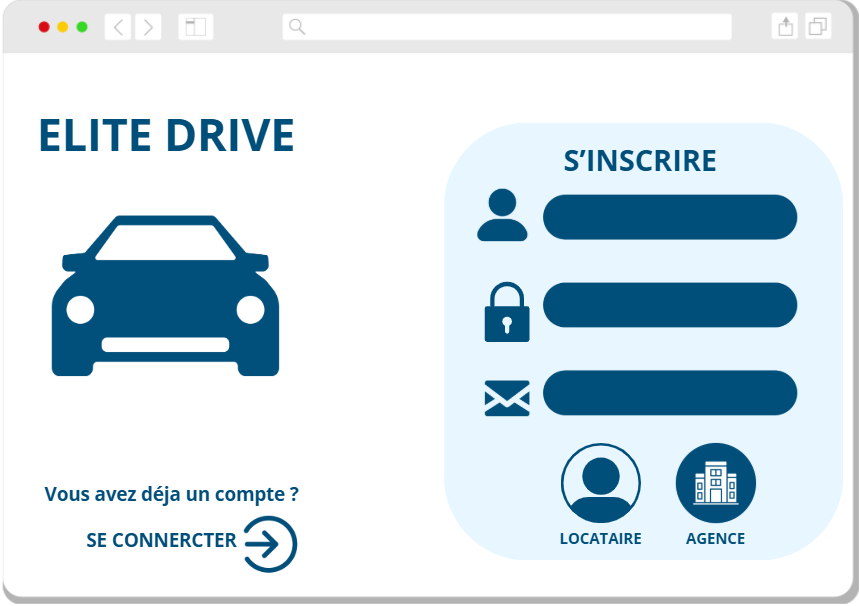
\includegraphics[width=0.8\textwidth]{Chapitres/Figures/proto_inscription.png}
    \caption{Prototypage de l'interface d'inscription}
    \label{fig:proto_inscription}
\end{figure}
\begin{figure}[H]
    \centering
    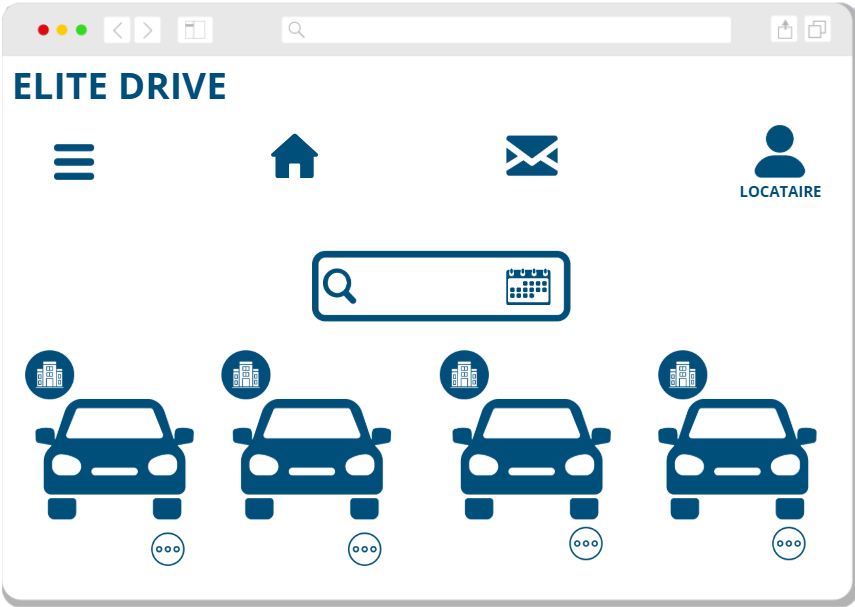
\includegraphics[width=0.8\textwidth]{Chapitres/Figures/proto_client.png}
    \caption{Prototypage de l'interface «Utilisateur»}
    \label{fig:proto_client}
\end{figure}

\clearpage
%%%%%%%%%%%%%%%%%%%%%%%%%%%%%%%%%%%%%%%%%%%%%%%%%%%%%%%%%%%%%%%%%%%%%%%%%%%
%section
\section{La spécification fonctionnelle des besoins}
\label{sec:besoins}
On décide d'étudier la spécification fonctionnelle en analysant les diagrammes de cas d'utilisation détaillés du premier sprint, ainsi que les descriptions textuelles et les diagrammes système associés à chaque fonctionnalité.

%%%%%%%%%%%%%%%%%%%%%%%%%%%%%%%%%%%%%%%%%%%%%%%%%%%%%%%%%%%%%%%%%%%%%%%%%%%
%section
\section{Diagramme de cas d'utilisation du premier sprint}
\label{sec:diag_cas_sprint1}
La figure suivante présente le diagramme des cas d'utilisation du premier sprint.
%%%%%%%%%%%%%%%%%%%%%%%%%%%%%%%%%%%%%%%%%%%%%%%%%%%%%%%%%%%%%%%
%figure
\begin{figure}[H]
    \centering
    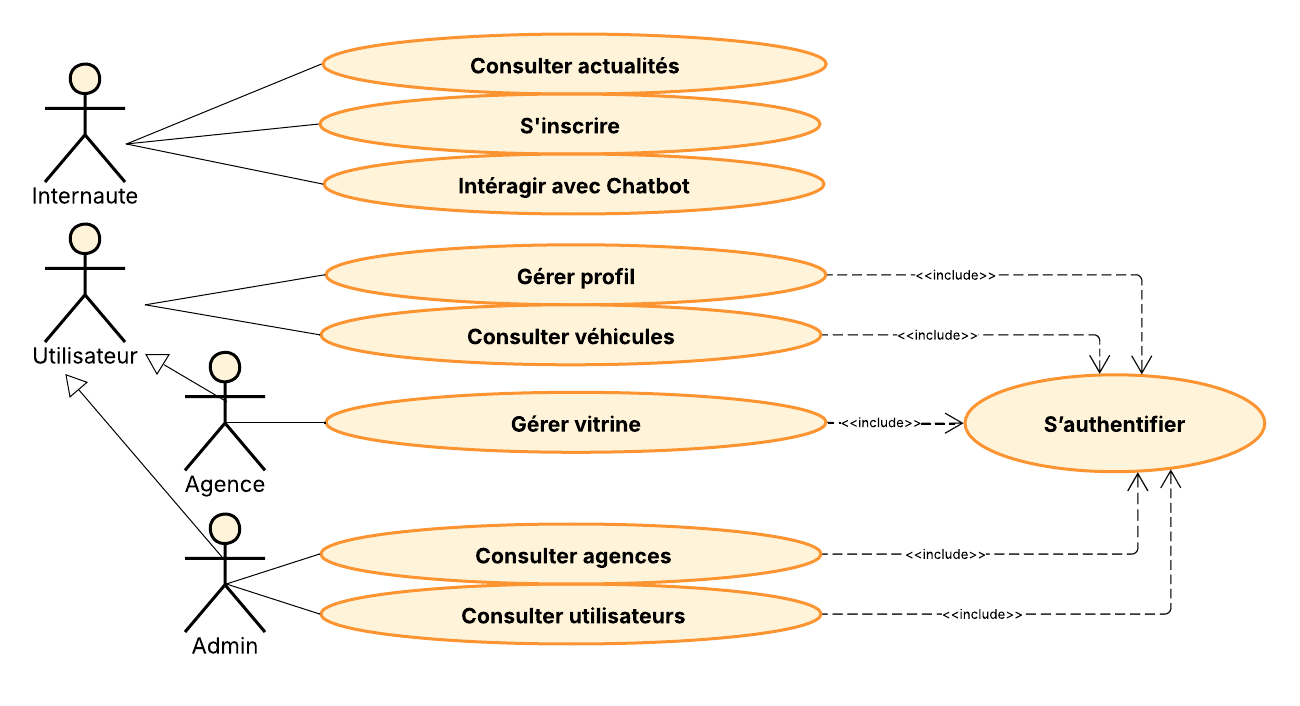
\includegraphics[width=1\textwidth]{Chapitres/Figures/diag_cas_sprint1.png}
    \caption{Diagramme de cas d'utilisation du premier sprint}
    \label{fig:Diag_use_case_S1}
\end{figure}
\newpage
\section{Analyse des cas d'utilisation du premier sprint}
\label{sec:sprint1}
À chaque cas d'utilisation, nous allons associer une description textuelle pour détailler le scénario ainsi que les éventuelles situations exceptionnelles.

%%%%%%%%%%%%%%%%%%%%%%%%%%%%%%%%%%%%%%%%%%%%%%%%%%%%%%%%%%%%%%%
\section{Analyse des cas d'utilisation de l'acteur «Internaute»}
\label{sec:use_case_acteur_internaute}
%%%%%%%%%%%%%%%%%%%%%%%%%%%%%%%%%%%%%%%%%%%%%%%%%%%%%%%%%%%%%%%
\subsection{Analyse de cas d'utilisation «Consulter actualités»}
\label{sec:cons_act}
Afin de mieux illustrer le déroulement du scénario, nous proposons ci‑après une description textuelle accompagnée du diagramme de séquence du cas d'utilisation \textbf{«Consulter actualités»}.
\begin{table}[H]
\centering
\caption{Description textuelle du cas d'utilisation «Consulter actualités»}
\label{tab:consulter_actualites}
\renewcommand{\arraystretch}{1.3}
\resizebox{\textwidth}{!}{%
\begin{tabular}{|l|p{11cm}|}
\hline
\textbf{Élément} & \textbf{Description} \\
\hline
Acteur & Internaute \\
\hline
Description & Permet à l’internaute de consulter les dernières actualités publiées sur la plateforme.\\
\hline
Précondition & L’internaute accède à la plateforme.\newline Des actualités sont disponibles. \\
\hline
Postcondition & L’internaute visualise les actualités.\newline Il peut accéder au détail d’une actualité. \\
\hline
Scénario nominal & 1. L’internaute accède à la section actualités.\newline
2. Le système affiche la liste des actualités.\newline
3. L’internaute sélectionne une actualité.\newline
4. Le système affiche le contenu détaillé. \\
\hline
Scénarios alternatifs & 
Pas d'exceptions\\
\hline
\end{tabular}
}
\end{table}
\begin{figure}[H]
    \centering
    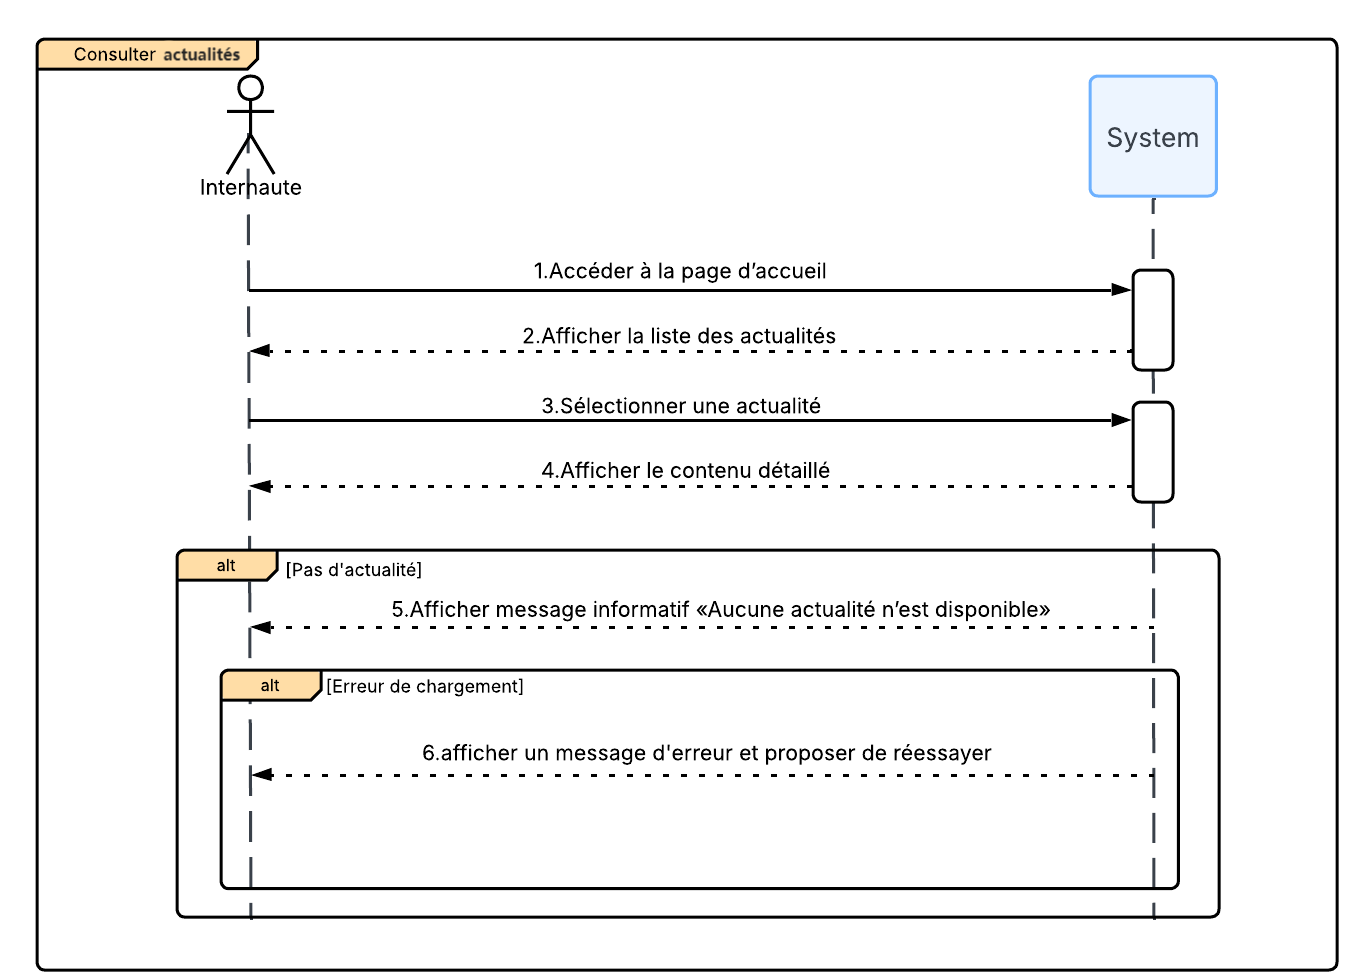
\includegraphics[width=0.7\textwidth]{Chapitres/Figures/Diag_seq_consulter_act.png}
    \caption{Diagramme de séquence système de cas d'utilisation «Consulter actualités»}
    \label{fig:consulter_actualites}
\end{figure}
%%%%%%%%%%%%%%%%%%%%%%%%%%%%%%%%%%%%%%%%%%%%%%%%%%%%%%%%%%%%%%%%
\subsection{Analyse de cas d'utilisation «S'inscrire»}
\label{sec:s_inscrire}
Afin de mieux illustrer le déroulement du scénario, nous proposons ci‑après une description textuelle accompagnée du diagramme de séquence du cas d'utilisation 
\textbf{«S'inscrire»}.

\begin{table}[htbp]
\centering
\caption{Description textuelle du cas d'utilisation «S'inscrire»}
\label{tab:s_inscrire}
\renewcommand{\arraystretch}{1.3}
\resizebox{\textwidth}{!}{%
\begin{tabular}{|l|p{11cm}|}
\hline
\textbf{Élément} & \textbf{Description} \\
\hline
Acteur & Internaute \\
\hline
Pré-condition & L'internaute consulte le site de l'application. \\
\hline
Post-condition & L'internaute est enregistré. \\
\hline
Scénario nominal &
1. L'internaute lance l'application. \newline
2. L'internaute sélectionne l'option «S'inscrire». \newline
3. Le système affiche le formulaire d'inscription. \newline
4. L'internaute remplit le formulaire. \newline
5. Le système vérifie les données saisies. \newline
6. L'internaute valide l'inscription. \newline
7. Le système vérifie l'unicité de l'e-mail. \newline
8. Le système redirige l'internaute vers le formulaire de connexion. \\
\hline
\multirow{9}{*}{\textbf{Scénario alternatif}} & 
5.1 Données manquantes ou incorrectes. \\
& \quad 5.1.1 Le système affiche un message d'erreur. \\
& \quad 5.1.2 Retour à l'étape 4 du scénario nominal. \\
& 5.2 Données invalides. \\
& \quad 5.2.1 Le système affiche un message d'erreur. \\
& \quad 5.2.2 Retour à l'étape 4 du scénario nominal. \\
& 7.1 Internaute déjà inscrit. \\
& \quad 7.1.1 Le système affiche un message d'erreur. \\
& \quad 7.1.2 Retour à l'étape 4 du scénario nominal. \\
\hline
\end{tabular}%
}
\end{table}

\begin{figure}[H]
    \centering
    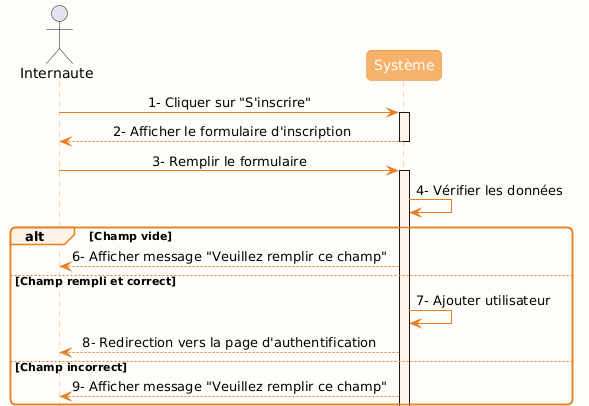
\includegraphics[width=0.7\textwidth]{Chapitres/Figures/diag_seq_s_inscrire.png}
    \caption{Diagramme de séquence système de cas d'utilisation «S'inscrire»}
    \label{fig:s_inscrire}
\end{figure}
%%%%%%%%%%%%%%%%


%%%%%%%%%%%%%%%%%%%%%%%%%%%%%%%%%%%%%%%%%%%%%%%%%%%%%%%%%%%%%%%
\subsection{Analyse de cas d'utilisation «Contacter administrateur»}
\label{sec:contacter_admin}
Afin de mieux illustrer le déroulement du scénario, nous proposons ci‑après une description textuelle accompagnée du diagramme de séquence du cas d'utilisation 
\textbf{«Contacter administrateur»}.

\begin{table}[htbp]
\centering
\caption{Description textuelle du cas d'utilisation «Contacter administrateur»}
\label{tab:contacter_admin}
\renewcommand{\arraystretch}{1.3}
\resizebox{\textwidth}{!}{%
\begin{tabular}{|l|p{11cm}|}
\hline
\textbf{Élément} & \textbf{Description} \\
\hline
Acteur & Internaute \\
\hline
Pré-condition & L'internaute accède au site de l'application. \newline
Le système est accessible. \\
\hline
Post-condition & Le message est envoyé à l’administrateur. \newline
Le système affiche un message de confirmation. \\
\hline
Scénario nominal &
1. L’internaute accède à la page «Contact». \newline
2. Le système affiche le formulaire de contact. \newline
3. L’internaute saisit les informations demandées et le message. \newline
4. L’internaute clique sur «Envoyer». \newline
5. Le système vérifie les données saisies. \newline
6. Le système envoie le message à l’administrateur. \newline
7. Le système affiche un message de confirmation. \\
\hline
\multirow{4}{*}{\textbf{Scénarios alternatifs}} 
& 5.1 Champs invalides ou incomplets. \\
& \quad 5.1.1 Le système affiche un message d’erreur. \\
& 6.1 Échec lors de l’envoi du message. \\
& \quad 6.1.1 Le système affiche un message d’échec. \\
\hline
\end{tabular}%
}
\end{table}

\begin{figure}[H]
    \centering
    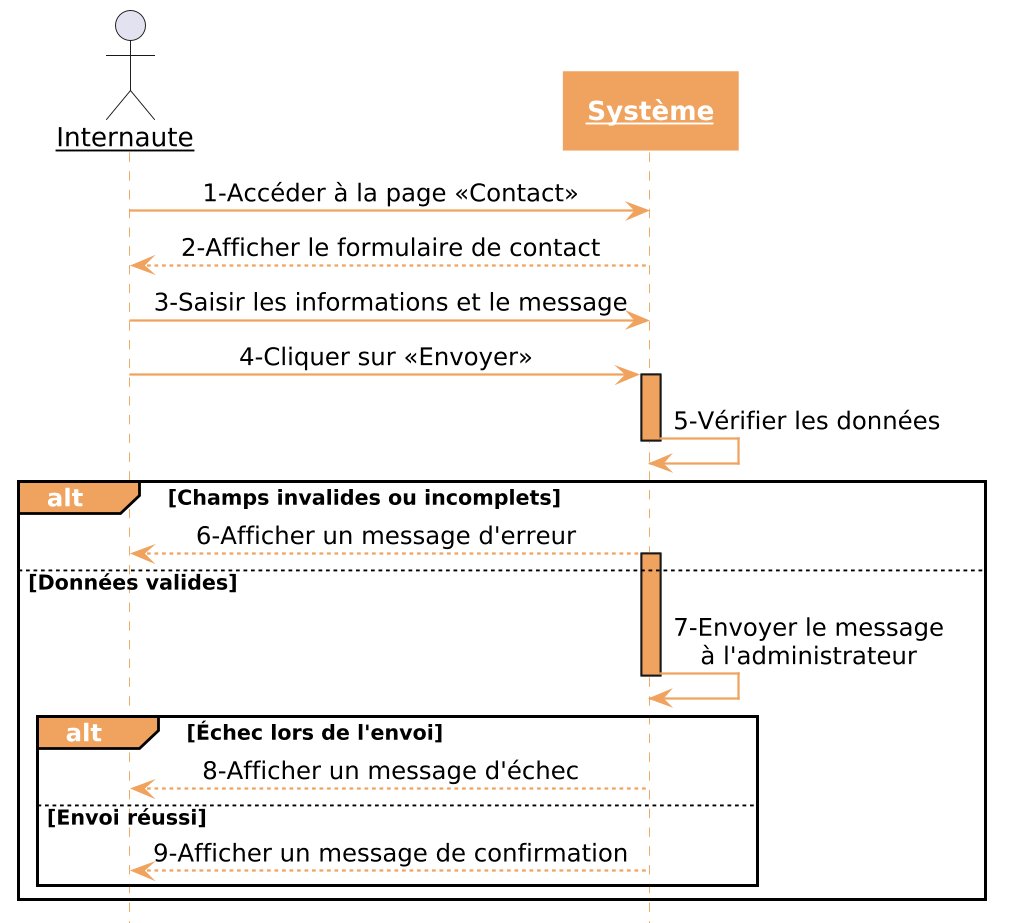
\includegraphics[width=0.7\textwidth]{Chapitres/Figures/diag_seq_contacter_admin.png}
    \caption{Diagramme de séquence système de cas d'utilisation «Contacter administrateur»}
    \label{fig:contacter_admin}
\end{figure}
%%%%%%%%%%%%%%%%%%%%%%%%%%%%%%%%%%%%%%%%%%%%%%%%%%%%%%%%%%%%%%%
\section{Analyse des cas d'utilisation de l'acteur «Utilisateur»}
\label{sec:acteur_utilisateur}
%%%%%%%%%%%%%%%%%%%%%%%%%%%%%%%%%%%%%%%%%%%%%%%%%%%%%%%%%%%%%%%
\subsection{Analyse de cas d'utilisation «S'authentifier»}
\label{sec:authentifier}
Afin de mieux illustrer le déroulement du scénario, nous proposons ci‑après une description textuelle accompagnée du diagramme de séquence du cas d'utilisation \textbf{«S'authentifier»}.
\begin{table}[htbp]
\centering
\caption{Description textuelle du cas d'utilisation «S'authentifier»}
\label{tab:authentifier}
\renewcommand{\arraystretch}{1.4}
\resizebox{\textwidth}{!}{%
\begin{tabular}{|l|p{11cm}|}
\hline
\textbf{Cas d'utilisation} & S'authentifier \\
\hline
\textbf{Acteur} & Utilisateur \\
\hline
\textbf{Pré-condition} & L'utilisateur a déjà un compte. \\
\hline
\textbf{Post-condition} & Utilisateur authentifié. \\
\hline
\multirow{8}{*}{\textbf{Scénario nominal}} & 1. L'utilisateur lance l'application.\\
& 2. L'utilisateur sélectionne l'option «Se connecter».\\
& 3. Le système fait apparaître le formulaire de connexion.\\
& 4. L'utilisateur entre son adresse de courrier électronique et son mot de passe.\\
& 5. Le système vérifie les données saisies.\\
& 6. L'utilisateur sélectionne l'option «Se connecter».\\
& 7. Le système examine la présence des informations saisies.\\
& 8. Le système redirige l'utilisateur vers son espace personnel.\\
\hline
\multirow{6}{*}{\textbf{Scénario alternatif}} & 5.1 L'utilisateur insère des données manquantes et/ou incorrectes.\\
& \quad 5.1.1 Le système fait apparaître un message d'erreur.\\
& \quad 5.1.2 Retour à l'étape 3 du scénario nominal.\\
& 5.2 Le compte est inexistant.\\
& \quad 5.2.1 Le système fait apparaître un message d'erreur.\\
& \quad 5.2.2 Retour à l'étape 3 du scénario nominal.\\
\hline
\end{tabular}%
}
\end{table}

\begin{figure}[H]
    \centering
    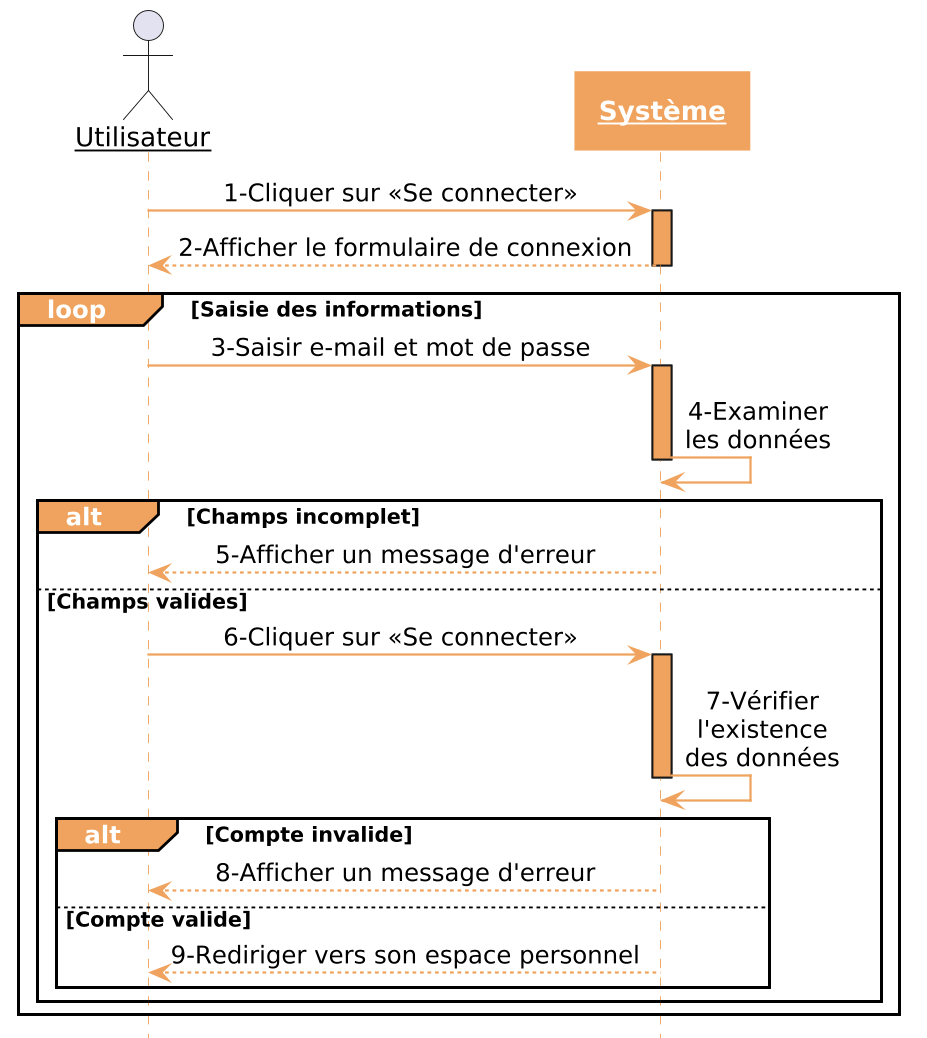
\includegraphics[width=1\textwidth]{Chapitres/Figures/diag_seq_s_authentifier.png}
    \caption{Diagramme de séquence système de cas d'utilisation «S'authentifier»}
    \label{fig:authentifier}
\end{figure}

%%%%%%%%%%%%%%%%%%%%%%%%%%%%%%%%%%%%%%%%%%%%%%%%%%%%
\newpage
\subsection{Analyse de cas d'utilisation «Gérer profil»}
\label{sec:gerer_profil}
La section suivante présente le raffinement du cas d’utilisation «Gérer profil» de l’acteur \textit{Utilisateur}.
\begin{figure}[H]
    \centering
    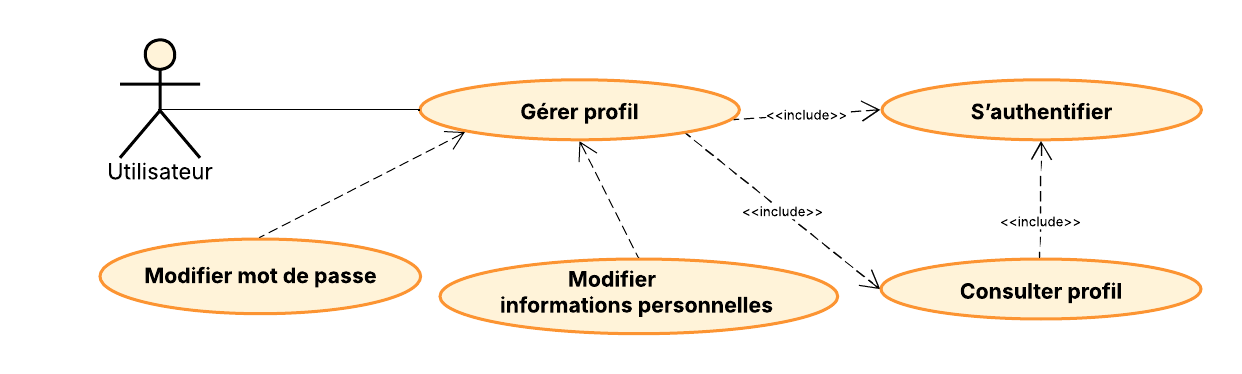
\includegraphics[width=1\textwidth]{Chapitres/Figures/Diag_cas_Gerer_profil.png}
    \caption{Raffinement du cas d'utilisation «Gérer profil»}
    \label{fig:Diag_gerer_profil}
\end{figure}


%%%%%%%%%%%%%%%%%%%%%%%%%%%%%
\subsubsection{Analyse de cas d'utilisation «Consulter profil»}
\label{sec:consulter_profil}
La section suivante propose une description textuelle et un diagramme de séquence, auxquels s'ajoute l'analyse du cas d'utilisation \textbf{«Consulter profil»} de l'acteur \textbf{Utilisateur}.

\begin{table}[htbp]
\centering
\caption{Description textuelle du cas d'utilisation «Consulter profil»}
\label{tab:consulter_profil}
\renewcommand{\arraystretch}{1.3}
\resizebox{\textwidth}{!}{%
\begin{tabular}{|l|p{11cm}|}
\hline
\textbf{Élément} & \textbf{Description} \\
\hline
Nom & Consulter profil \\
\hline
Acteur & Utilisateur \\
\hline
Description brève & Permet à un utilisateur de consulter son profil. \\
\hline
Précondition & 
L'utilisateur est authentifié. \newline
Le système est accessible. \\
\hline
Postcondition & 
Ensemble des données affichés. \\
\hline
Enchaînement principal & 
1. L'utilisateur clique sur «Profil». \newline
2. Le système affiche les informations du profil. \\
\hline
Scénarios alternatifs & 
Pas d'exceptions\\
\hline
\end{tabular}%
}
\end{table}

\begin{figure}[H]
    \centering
    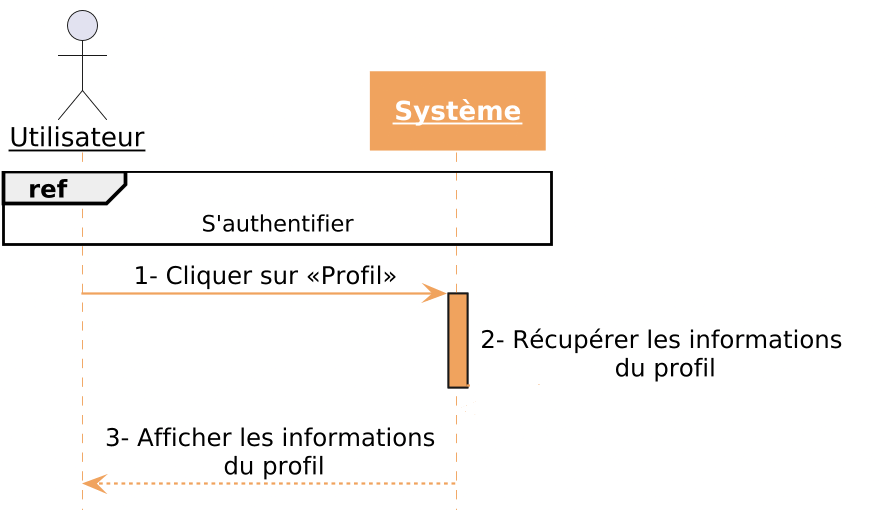
\includegraphics[width=0.7\textwidth]{Chapitres/Figures/diag_seq_consulter_profil.png}
    \caption{Diagramme de séquence système de cas d'utilisation «Consulter profil»}
    \label{fig:consulter_profil}
\end{figure}

\subsubsection{Analyse de cas d'utilisation «Modifier profil»}
\label{sec:modifier_profil}
La section suivante propose une description textuelle et un diagramme de séquence, auxquels s'ajoute l'analyse du cas d'utilisation \textbf{«Modifier profil»} de l'acteur \textbf{Utilisateur}.

\begin{table}[htbp]
\centering
\caption{Description textuelle du cas d'utilisation «Modifier profil»}
\label{tab:modifier_profil}
\renewcommand{\arraystretch}{1.3}
\resizebox{\textwidth}{!}{%
\begin{tabular}{|l|p{11cm}|}
\hline
\textbf{Élément} & \textbf{Description} \\
\hline
Nom & Modifier profil \\
\hline
Acteur & Utilisateur \\
\hline
Description brève & Permet à un utilisateur de modifier ses informations personnelles (nom, email, mot de passe, numéro de téléphone). \\
\hline
Précondition & 
L'utilisateur est authentifié. \newline
Le système est accessible. \\
\hline
Postcondition & 
Les informations du profil sont mises à jour. \newline
Les nouvelles données sont enregistrées. \\
\hline
Enchaînement principal & 
1. L'utilisateur accède à la page «profil». \newline
2. Le système affiche les informations actuelles du profil. \newline
3. L'utilisateur modifie ses informations personnelles. \newline
4. Le système vérifie les données et effectue la modification. \newline
5. Le système affiche un message de confirmation. \\
\hline
\multirow{4}{*}{\textbf{Scénarios alternatifs}} 
& 4.1 Informations invalides. \\
& \quad 4.1.1 Le système affiche un message d'erreur. \\
& 5.1 Échec lors de l'enregistrement. \\
& \quad 5.1.1 Le système affiche un message d'échec. \\
\hline
\end{tabular}%
}
\end{table}
\begin{figure}[H]
    \centering
    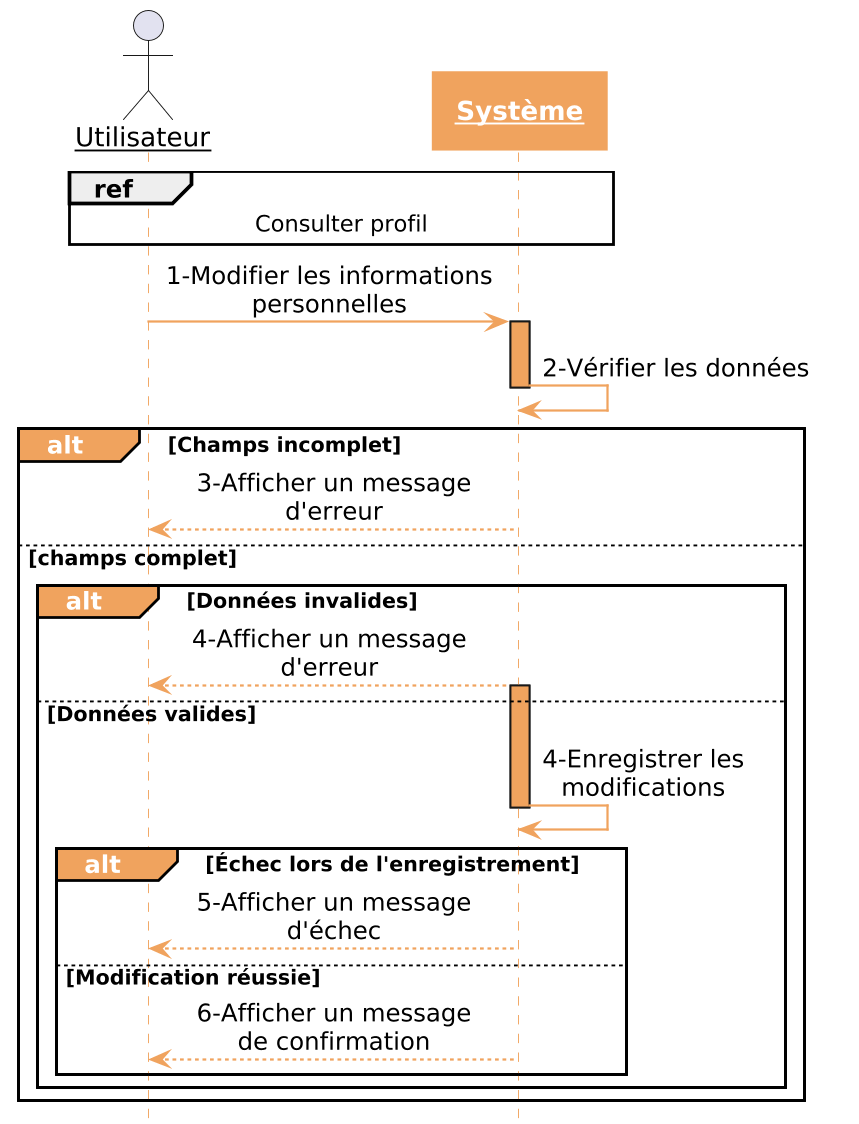
\includegraphics[width=0.7\textwidth]{Chapitres/Figures/diag_seq_modifier_profil.png}
    \caption{Diagramme de séquence système de cas d'utilisation «Modifier profil»}
    \label{fig:modifier_profil}
\end{figure}

%%%%%%%%%%%%%%%%%%%%%%%%%%%%%
%%%%%%1111%%%%%%%%%


%%%%%%%%%%44444444444%%%%%%%%%%%%%%%%%%%%%%%%
\FloatBarrier
\section{Analyse des cas d'utilisation de l'acteur «Administrateur»}
\label{sec:acteur_admin}
%%%%%%%%%%%%%%%%%%%%%%%%%%%%%%%%%%%%%%%%%%%%%%%%%%%%%%%%%%%%%%%

\subsection{Analyse de cas d'utilisation «Gérer agences»}
\label{sec:gerer_agences}
Afin de mieux illustrer le déroulement du scénario, nous proposons ci‑après un raffinement du cas d'utilisation \textbf{«Gérer agences»} de l'acteur \textit{Administrateur}.

\begin{figure}[H]
    \centering
    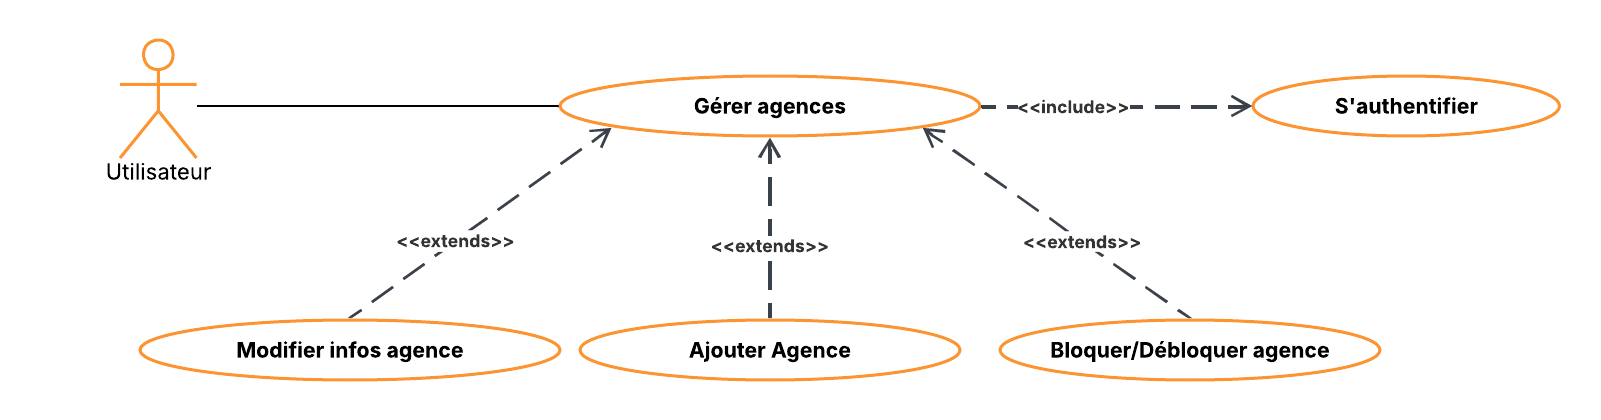
\includegraphics[width=1\textwidth]{Chapitres/Figures/raf_gerer_agences.png}
    \caption{Raffinement du cas d'utilisation «Gérer agences»}
    \label{fig:raf_gerer_agences}
\end{figure}
%%%%%%%%%%%%%%
\subsubsection{Analyse de cas d'utilisation «Consulter agences»}
\label{sec:consulter_agences}
La section suivante propose une description textuelle et un diagramme de séquence, auxquels s'ajoute l'analyse du cas d'utilisation \textbf{«Consulter agences»} de l'acteur \textbf{Administrateur}.

\begin{table}[htbp]
\centering
\caption{Description textuelle du cas d'utilisation «Consulter agences»}
\label{tab:consulter_agences}
\renewcommand{\arraystretch}{1.3}
\resizebox{\textwidth}{!}{%
\begin{tabular}{|l|p{11cm}|}
\hline
\textbf{Élément} & \textbf{Description} \\
\hline
Nom & Consulter agences \\
\hline
Acteur & Administrateur \\
\hline
Description brève & Permet à un administrateur de consulter les informations des agences. \\
\hline
Précondition & 
L'administrateur est authentifié. \newline
Le système est accessible. \\
\hline
Postcondition & 
Ensemble des données affichés. \\
\hline
Enchaînement principal & 
1. L'administrateur clique sur «Agences». \newline
2. Le système affiche les informations des agences. \\
\hline
Scénarios alternatifs & 
Pas d'exceptions\\
\hline
\end{tabular}%
}
\end{table}

\begin{figure}[H]
    \centering
    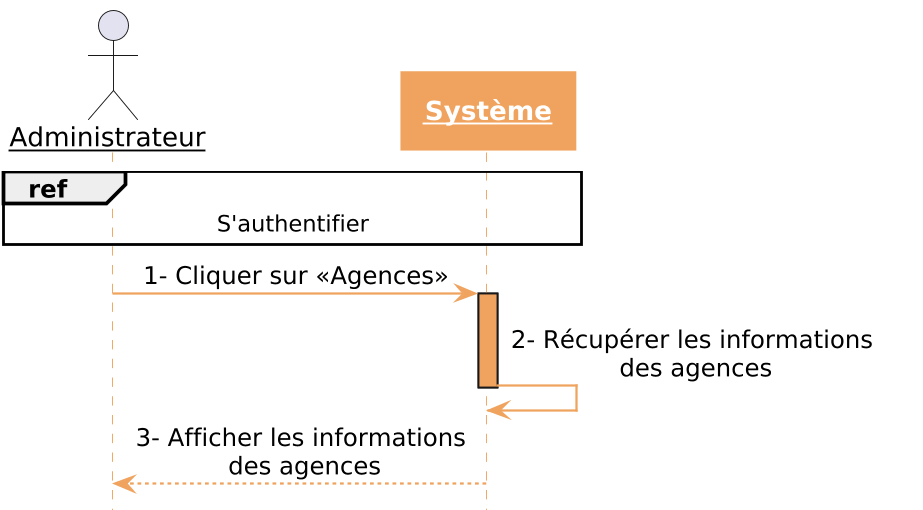
\includegraphics[width=0.7\textwidth]{Chapitres/Figures/diag_seq_consulter_agences.png}
    \caption{Diagramme de séquence système de cas d'utilisation «Consulter agences»}
    \label{fig:consulter_agences}
\end{figure}

%%%%%%%%%%%%%%
\subsubsection{Analyse de cas d'utilisation «Modifier infos agence»}
\label{sec:modifier_infos_agence}
La section suivante propose une description textuelle et un diagramme de séquence, auxquels s'ajoute l'analyse du cas d'utilisation \textbf{«Modifier infos agence»} de l'acteur \textbf{Administrateur}.

\begin{table}[htbp]
\centering
\caption{Description textuelle du cas d'utilisation «Modifier infos agence»}
\label{tab:modifier_infos_agence}
\renewcommand{\arraystretch}{1.3}
\resizebox{\textwidth}{!}{%
\begin{tabular}{|l|p{11cm}|}
\hline
\textbf{Élément} & \textbf{Description} \\
\hline
Nom & Modifier infos agence \\
\hline
Acteur & Administrateur \\
\hline
Description brève & Permet à un administrateur de modifier les informations d'une agence. \\
\hline
Précondition & 
L'administrateur est authentifié. \newline
Le système est accessible. \\
\hline
Postcondition & 
Les informations de l'agence sont mises à jour. \newline
Les nouvelles données sont enregistrées. \\
\hline
Enchaînement principal & 
1. L'administrateur accède à la page «gestion des agences». \newline
2. Le système affiche les informations actuelles de l'agence. \newline
3. L'administrateur modifie les informations de l'agence. \newline
4. Le système vérifie les données et effectue la modification. \newline
5. Le système affiche un message de confirmation. \\
\hline
\multirow{4}{*}{\textbf{Scénarios alternatifs}} 
& 4.1 Informations invalides. \\
& \quad 4.1.1 Le système affiche un message d'erreur. \\
& 5.1 Échec lors de l'enregistrement. \\
& \quad 5.1.1 Le système affiche un message d'échec. \\
\hline
\end{tabular}%
}
\end{table}
\begin{figure}[H]
    \centering
    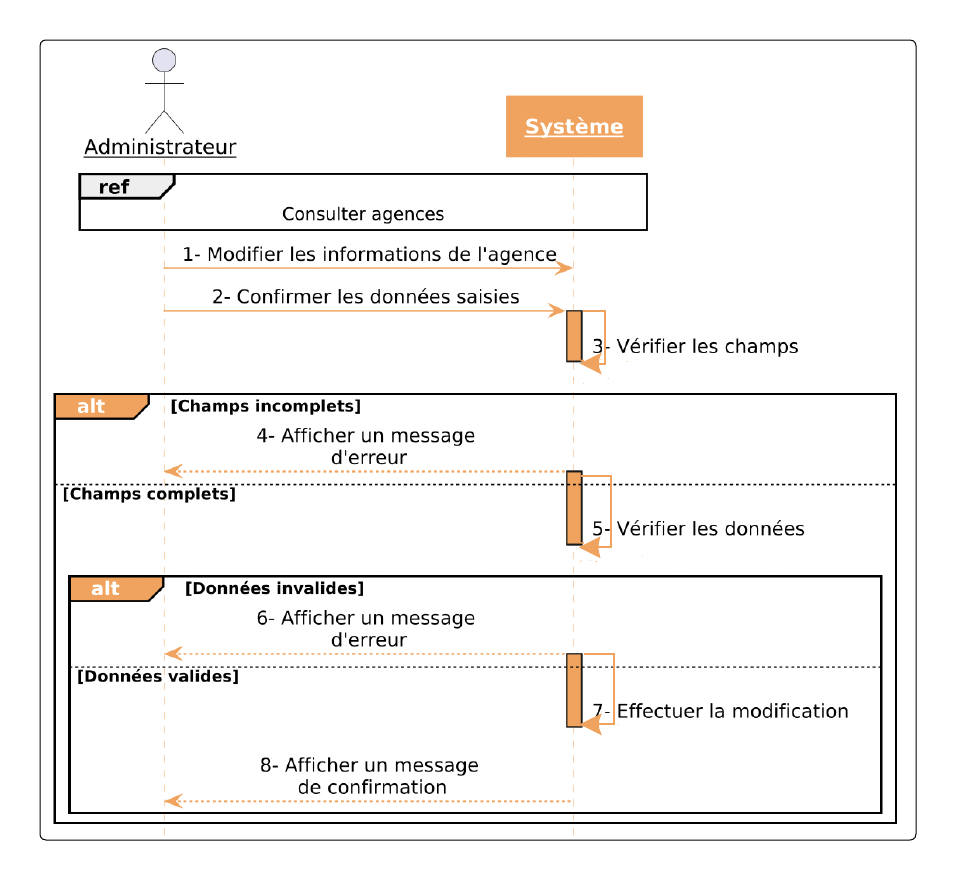
\includegraphics[width=0.7\textwidth]{Chapitres/Figures/diag_seq_modifier_infos_agences.png}
    \caption{Diagramme de séquence système de cas d'utilisation «Modifier infos agence»}
    \label{fig:modifier_infos_agences}
\end{figure}

%%%%%%%%%%%%%%%%    
\FloatBarrier
\subsection{Analyse de cas d'utilisation «Ajouter agence»}
\label{sec:ajouter_agence}
Dans la suite, nous présentons une description textuelle accompagnée d'un diagramme 
de séquence du cas d'utilisation \textbf{«Ajouter agence»} de l'acteur 
\textbf{Administrateur}.
\begin{table}[htbp]
\centering
\caption{Description textuelle du cas d'utilisation «Ajouter agence»}
\label{tab:ajouter_agence}
\renewcommand{\arraystretch}{1.3}
\resizebox{\textwidth}{!}{%
\begin{tabular}{|l|p{11cm}|}
\hline
\textbf{Élément} & \textbf{Description} \\
\hline
Nom & ajouter agence \\
\hline
Acteur & Administrateur \\
\hline
Description brève & Permet à l'administrateur d'ajouter une agence. \\
\hline
Précondition & 
 L'administrateur est authentifié. \newline
 Le système est accessible. \\
\hline
Postcondition & 
 Une agence est ajoutée. \\
\hline
Enchaînement principal & 
1. L'administrateur accède à la page de gestion. \newline
2. Le système affiche la liste des agence. \newline
3. L'administrateur clique sur «ajouter une agence». \newline
4. Le système affiche le formulaire d'ajout. \newline
5. L'administrateur saisit les informations nécessaires. \newline
6. Le système vérifie les données. \newline
7. Le système enregistre l'agence. \newline
8. Le système affiche un message de confirmation. \\
\hline
\multirow{6}{*}{\textbf{Scénario alternatif}} & 6.1 Informations invalides.\\
& \quad 6.1.1 Le système affiche un message d'erreur. \\
& 7.1 Erreur lors de l'enregistrement. \\
& \quad 7.1.1 Le système affiche un message d'échec. \\
\hline
\end{tabular}%
}
\end{table}

\begin{figure}[H]
    \centering
    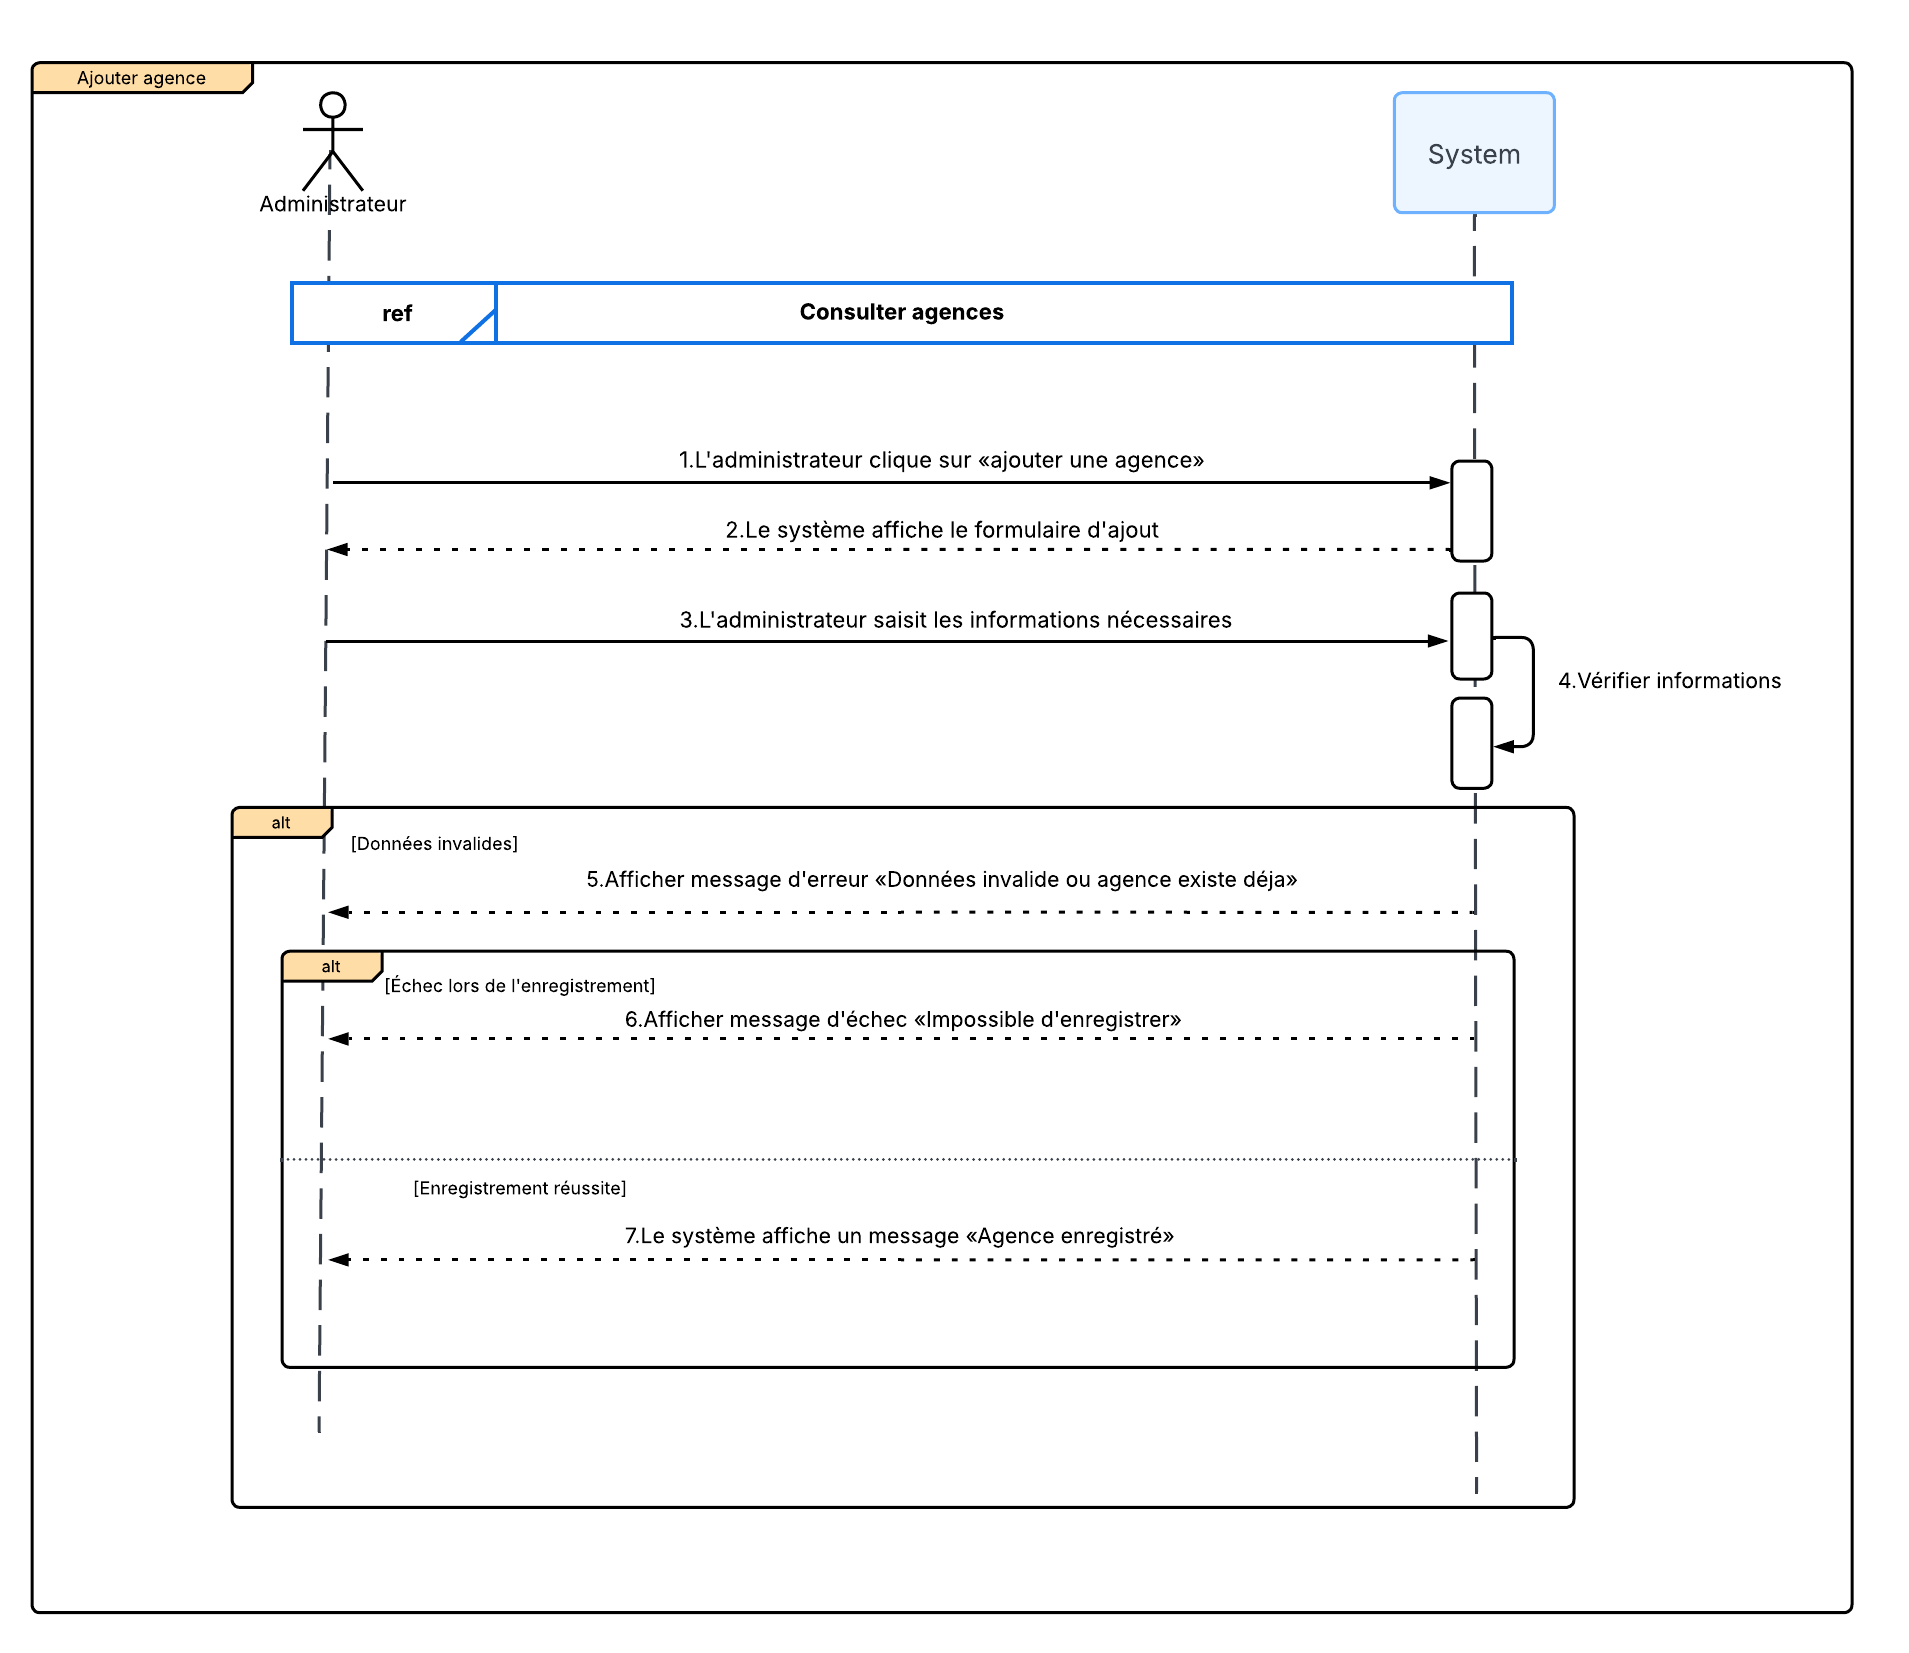
\includegraphics[width=1\textwidth]{Chapitres/Figures/Diag_seq_ajouter_agence.png}
    \caption{Diagramme de séquence système de cas d'utilisation «Ajouter agence»}
    \label{fig:ajouter_agence}
\end{figure}

\FloatBarrier
\subsection{Analyse de cas d'utilisation «Bloquer/Débloquer agence»}
\label{sec:bloquer/debloquer_agence}
Dans la suite, nous présentons une description textuelle accompagnée d'un diagramme 
de séquence du cas d'utilisation \textbf{«Bloquer/Débloquer agence»} de l'acteur 
\textbf{Administrateur}.

\begin{table}[H]
\centering
\caption{Description textuelle du cas d'utilisation «Bloquer/Débloquer agence»}
\label{tab:use-case-bloquer-agence}
\renewcommand{\arraystretch}{1.3}
\begin{tabular}{|l|p{10cm}|}
\hline
\textbf{Élément} & \textbf{Description} \\
\hline
Nom & Bloquer/Débloquer agence \\
\hline
Acteur & Administrateur \\
\hline
Description brève & Permet à l'administrateur de bloquer ou de débloquer une agence afin de désactiver ou d'activer son accès. \\
\hline
Précondition & 
 L'administrateur est authentifié. \newline
 L'agence existe dans le système. \\
\hline
Postcondition & 
 L'agence est bloquée/Débloquée et peut/ ne peut plus accéder au système. \\
\hline
Enchaînement principal & 
1. L'administrateur consulte la liste des agences. \newline
2. L'administrateur sélectionne une agence. \newline
3. L'administrateur clique sur «Bloquer/Débloquer». \newline
4. Le système demande confirmation. \newline
5. L'administrateur confirme. \newline
6. Le système bloque/débloque l'agence. \newline
7. Le système affiche un message de confirmation. \\
\hline
\multirow{4}{*}{\textbf{Scénario alternatif}} 
& 5.1 Annulation de l'action. \\
& \quad 5.1.1 Aucune modification n'est effectuée. \\
& 6.1 Erreur lors du blocage/déblocage. \\
& \quad 6.1.1 Le système affiche un message d'échec. \\
\hline
\end{tabular}
\end{table}

\begin{figure}[H]
    \centering
    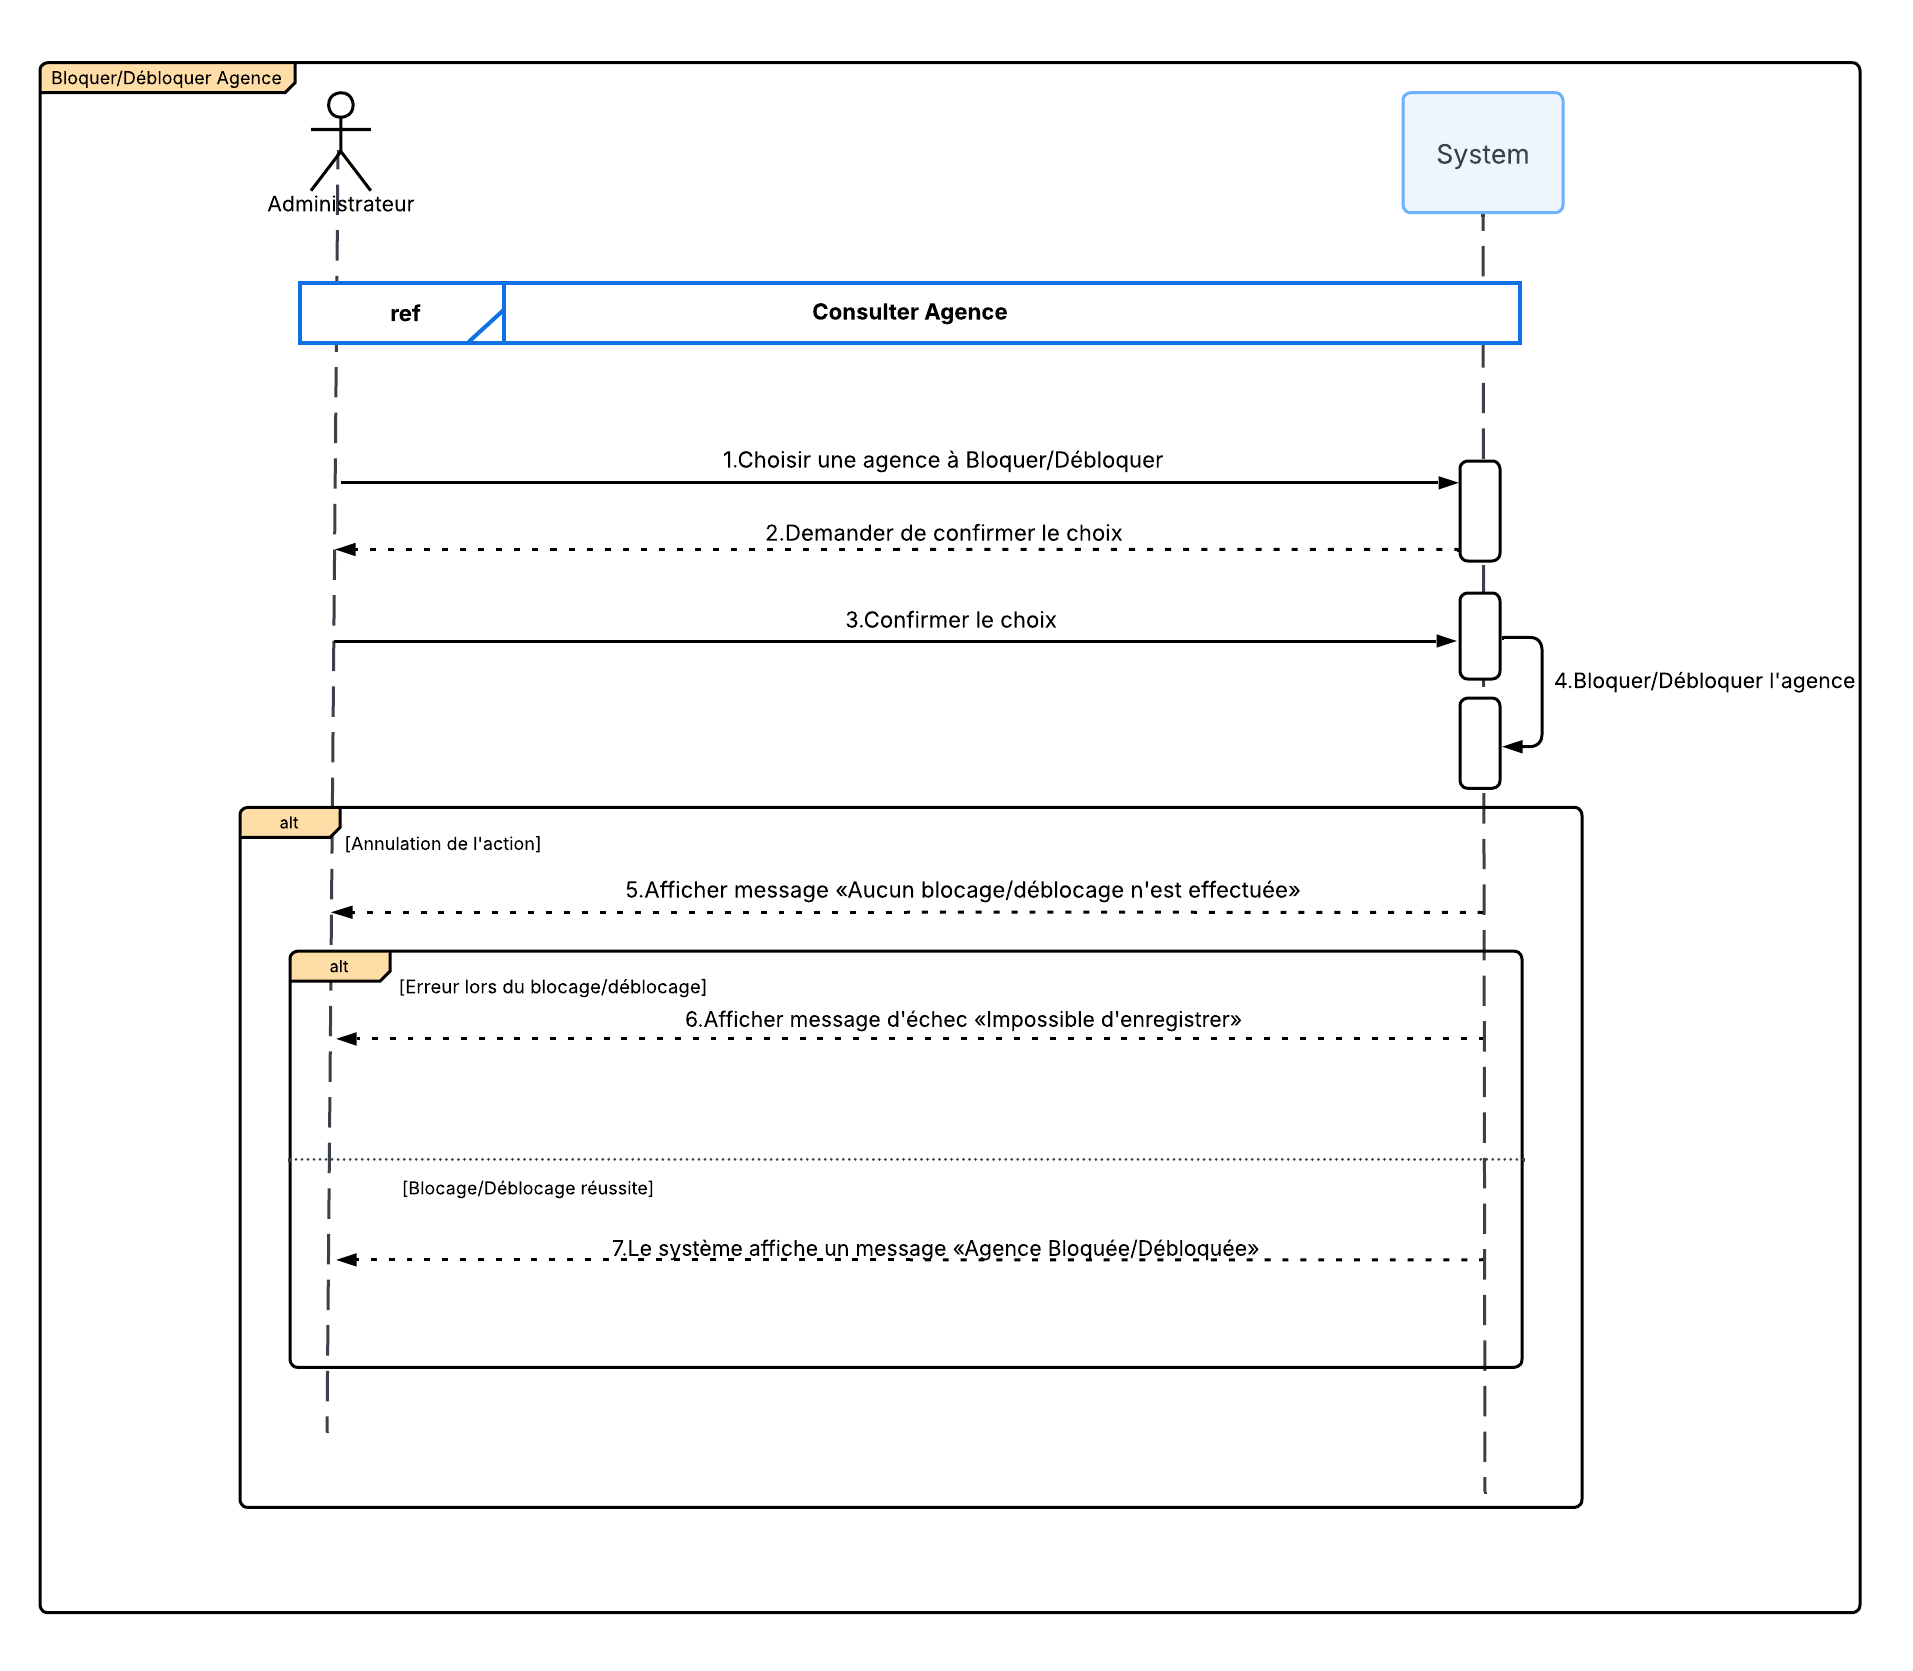
\includegraphics[width=1\textwidth]{Chapitres/Figures/Diag_seq_bloquer_agence.png}
    \caption{Diagramme de séquence système de cas d'utilisation «Bloquer agences»}
    \label{fig:bloquer_agences}
\end{figure}

\subsection{Analyse de cas d'utilisation "Gérer messages''}
\label{sec:gerer_messages}

Afin de mieux illustrer le déroulement du scénario, nous proposons ci-après une analyse
du cas d'utilisation "\textbf{Gérer messages}'' de l'acteur Administrateur.

\begin{table}[H]
\centering
\caption{Description textuelle du cas d'utilisation "Gérer messages''}
\label{tab:gerer_messages}
\renewcommand{\arraystretch}{1.35}
\begin{tabular}{|p{3.5cm}|p{10cm}|}
\hline
\textbf{Élément} & \textbf{Description} \\
\hline
Nom & Gérer messages \\
\hline
Acteur & Administrateur \\
\hline
Description brève & Permet à l'administrateur de consulter les messages reçus des utilisateurs et d'y apporter une réponse. \\
\hline
Précondition & L'administrateur est authentifié. \newline
               Le système est accessible. \\
\hline
Postcondition & Le message est traité et une réponse est envoyée à l'utilisateur concerné. \\
\hline
Enchaînement principal &
1. L'administrateur accède à la section "~Messages~''. \newline
2. Le système affiche la liste des messages reçus avec leur statut. \newline
3. L'administrateur sélectionne un message. \newline
4. Le système affiche le contenu du message et les informations de l'expéditeur. \newline
5. L'administrateur rédige une réponse. \newline
6. Le système enregistre et envoie la réponse. \newline
7. Le système marque le message comme traité et affiche un message de confirmation. \\
\hline
\textbf{Scénario alternatif} &
6.1 Erreur lors de l'envoi de la réponse. \newline
\quad 6.1.1 Le système affiche un message d'échec. \\
\hline
\end{tabular}
\end{table}

\begin{figure}[H]
    \centering
    
\includegraphics[width=1\textwidth]{Chapitres/figures/seq_gerer_messages.png}
    \caption{Diagramme de séquence système de cas d'utilisation "Gérer messages''}
    \label{fig:seq_gerer_messages}
\end{figure}

%%%%%%%%%%%%%%%%%%%%%%%%%%%%%%%%%%%%%%%%%%%%%%%%%%%%%%%%%%%%%%%
\newpage
\FloatBarrier
\section{Analyse des cas d'utilisation de l'acteur «Agence»}
\label{sec:acteur_agence}
%%%%%%%%%%%%%%%%%%%%%%%%%%%%%%%%%%%%%%%%%%%%%%%%%%%%%%%%%%%%%%%

\subsection{Analyse de cas d'utilisation «Gérer vitrine»}
\label{sec:gerer_vitrine}
Pour mieux analyser le déroulement du scénario, nous proposons ci‑après un 
raffinement accompagné d'une description textuelle et un diagramme de séquence du cas d'utilisation \textbf{«Gérer vitrine»} de l'acteur \textit{Agence}.

\begin{figure}[H]
    \centering
    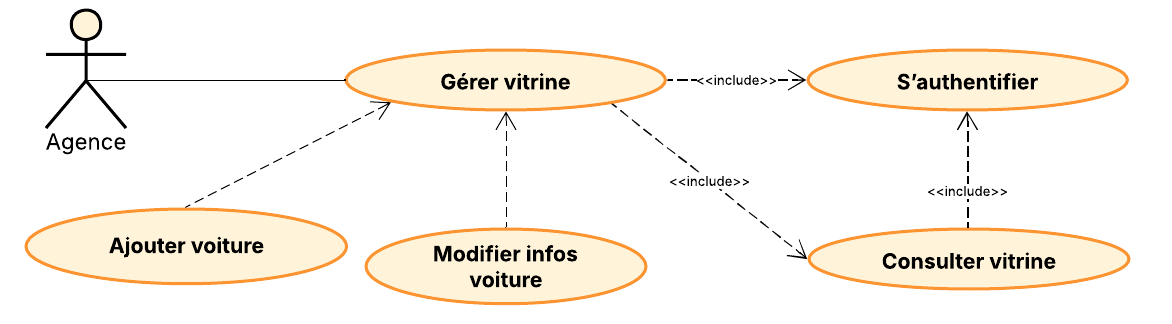
\includegraphics[width=1\textwidth]{Chapitres/Figures/raf_gerer_vitrine.png}
    \caption{Raffinement du cas d'utilisation «Gérer vitrine»}
    \label{fig:raf_gerer_vitrine}
\end{figure}

\subsubsection{Analyse de cas d'utilisation «Consulter vitrine»}
\label{sec:consulter_vitrine}
La section suivante propose une description textuelle et une diagramme de séquence, auxquels s'ajoute l'analyse du cas d'utilisation \textbf{«Consulter vitrine»} de l'acteur \textit{Agence}.

\begin{table}[htbp]
\centering
\caption{Description textuelle du cas d'utilisation «Consulter vitrine»}
\label{tab:consulter_vitrine}
\renewcommand{\arraystretch}{1.3}
\resizebox{\textwidth}{!}{%
\begin{tabular}{|l|p{11cm}|}
\hline
\textbf{Élément} & \textbf{Description} \\
\hline
Nom & Consulter vitrine \\
\hline
Acteur & Agence \\
\hline
Description brève & Permet à une agence de consulter sa vitrine. \\
\hline
Précondition & 
L'agence est authentifié. \newline
Le système est accessible. \\
\hline
Postcondition & 
La liste des voitures est affichés ainsi que leurs informations. \\
\hline
Enchaînement principal & 
1. L'Agence clique sur «vitrine». \newline
2. Le système affiche les voitures enregistrées dans la vitrine ainsi que leurs informations. \\
\hline
Scénarios alternatifs & 
pas d'exceptions\\
\hline
\end{tabular}%
}
\end{table}

\begin{figure}[H]
    \centering
    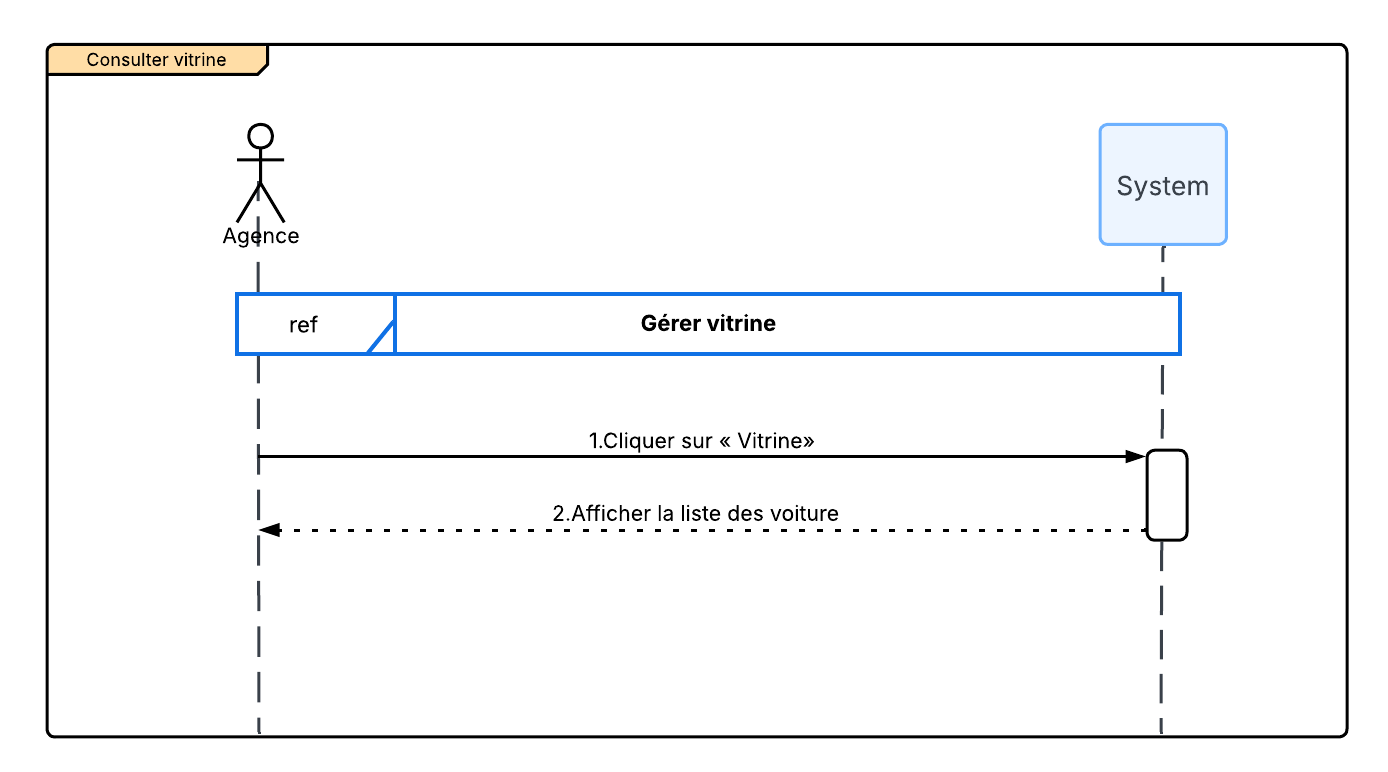
\includegraphics[width=0.7\textwidth]{Chapitres/Figures/Diag_seq_consulter_vitrine.png}
    \caption{Diagramme de séquence système de cas d'utilisation «Consulter vitrine»}
    \label{fig:consulter_vitrine}
\end{figure}
%%%%%%%%%%%%%%%%
\subsubsection{Analyse de cas d'utilisation «Modifier informations voiture»}
\label{sec:modifier_infos_voiture}
La section suivante propose une description textuelle et un diagramme de séquence, auxquels s'ajoute l'analyse du cas d'utilisation \textbf{«Modifier informations voiture»} de l'acteur \textbf{Agence}.


\begin{table}[htbp]
\centering
\caption{Description textuelle du cas d'utilisation «Modifier informations voiture»}
\label{tab:modifier_infos_voiture}
\renewcommand{\arraystretch}{1.3}
\resizebox{\textwidth}{!}{%
\begin{tabular}{|l|p{11cm}|}
\hline
\textbf{Élément} & \textbf{Description} \\
\hline
Nom & Modifier informations voiture \\
\hline
Acteur & Agence \\
\hline
Description brève & Permet à un Agence de consulter et de modifier ses informations voiture (nom, email, adresse, numéro de téléphone). \\
\hline
Précondition & 
L'agence est authentifié. \newline
Le système est accessible. \\
\hline
Postcondition & 
Les informations du voiture sont mises à jour. \newline
Les nouvelles données sont enregistrées. \\
\hline
Enchaînement principal & 
1. L'agence accède à la page «vitrine». \newline
2. Le système affiche les voiture actuelles. \newline
3. L'agence modifie les informations d'une voiture. \newline
4. Le système vérifie les données et effectue l'action. \newline
5. Le système affiche un message de confirmation. \\
\hline
\multirow{4}{*}{\textbf{Scénarios alternatifs}} 
& 4.1 Informations invalides. \\
& \quad 4.1.1 Le système affiche un message d'erreur. \\
& 5.1 Échec lors de l'enregistrement. \\
& \quad 5.1.1 Le système affiche un message d'échec. \\
\hline
\end{tabular}%
}
\end{table}
\begin{figure}[H]
    \centering
    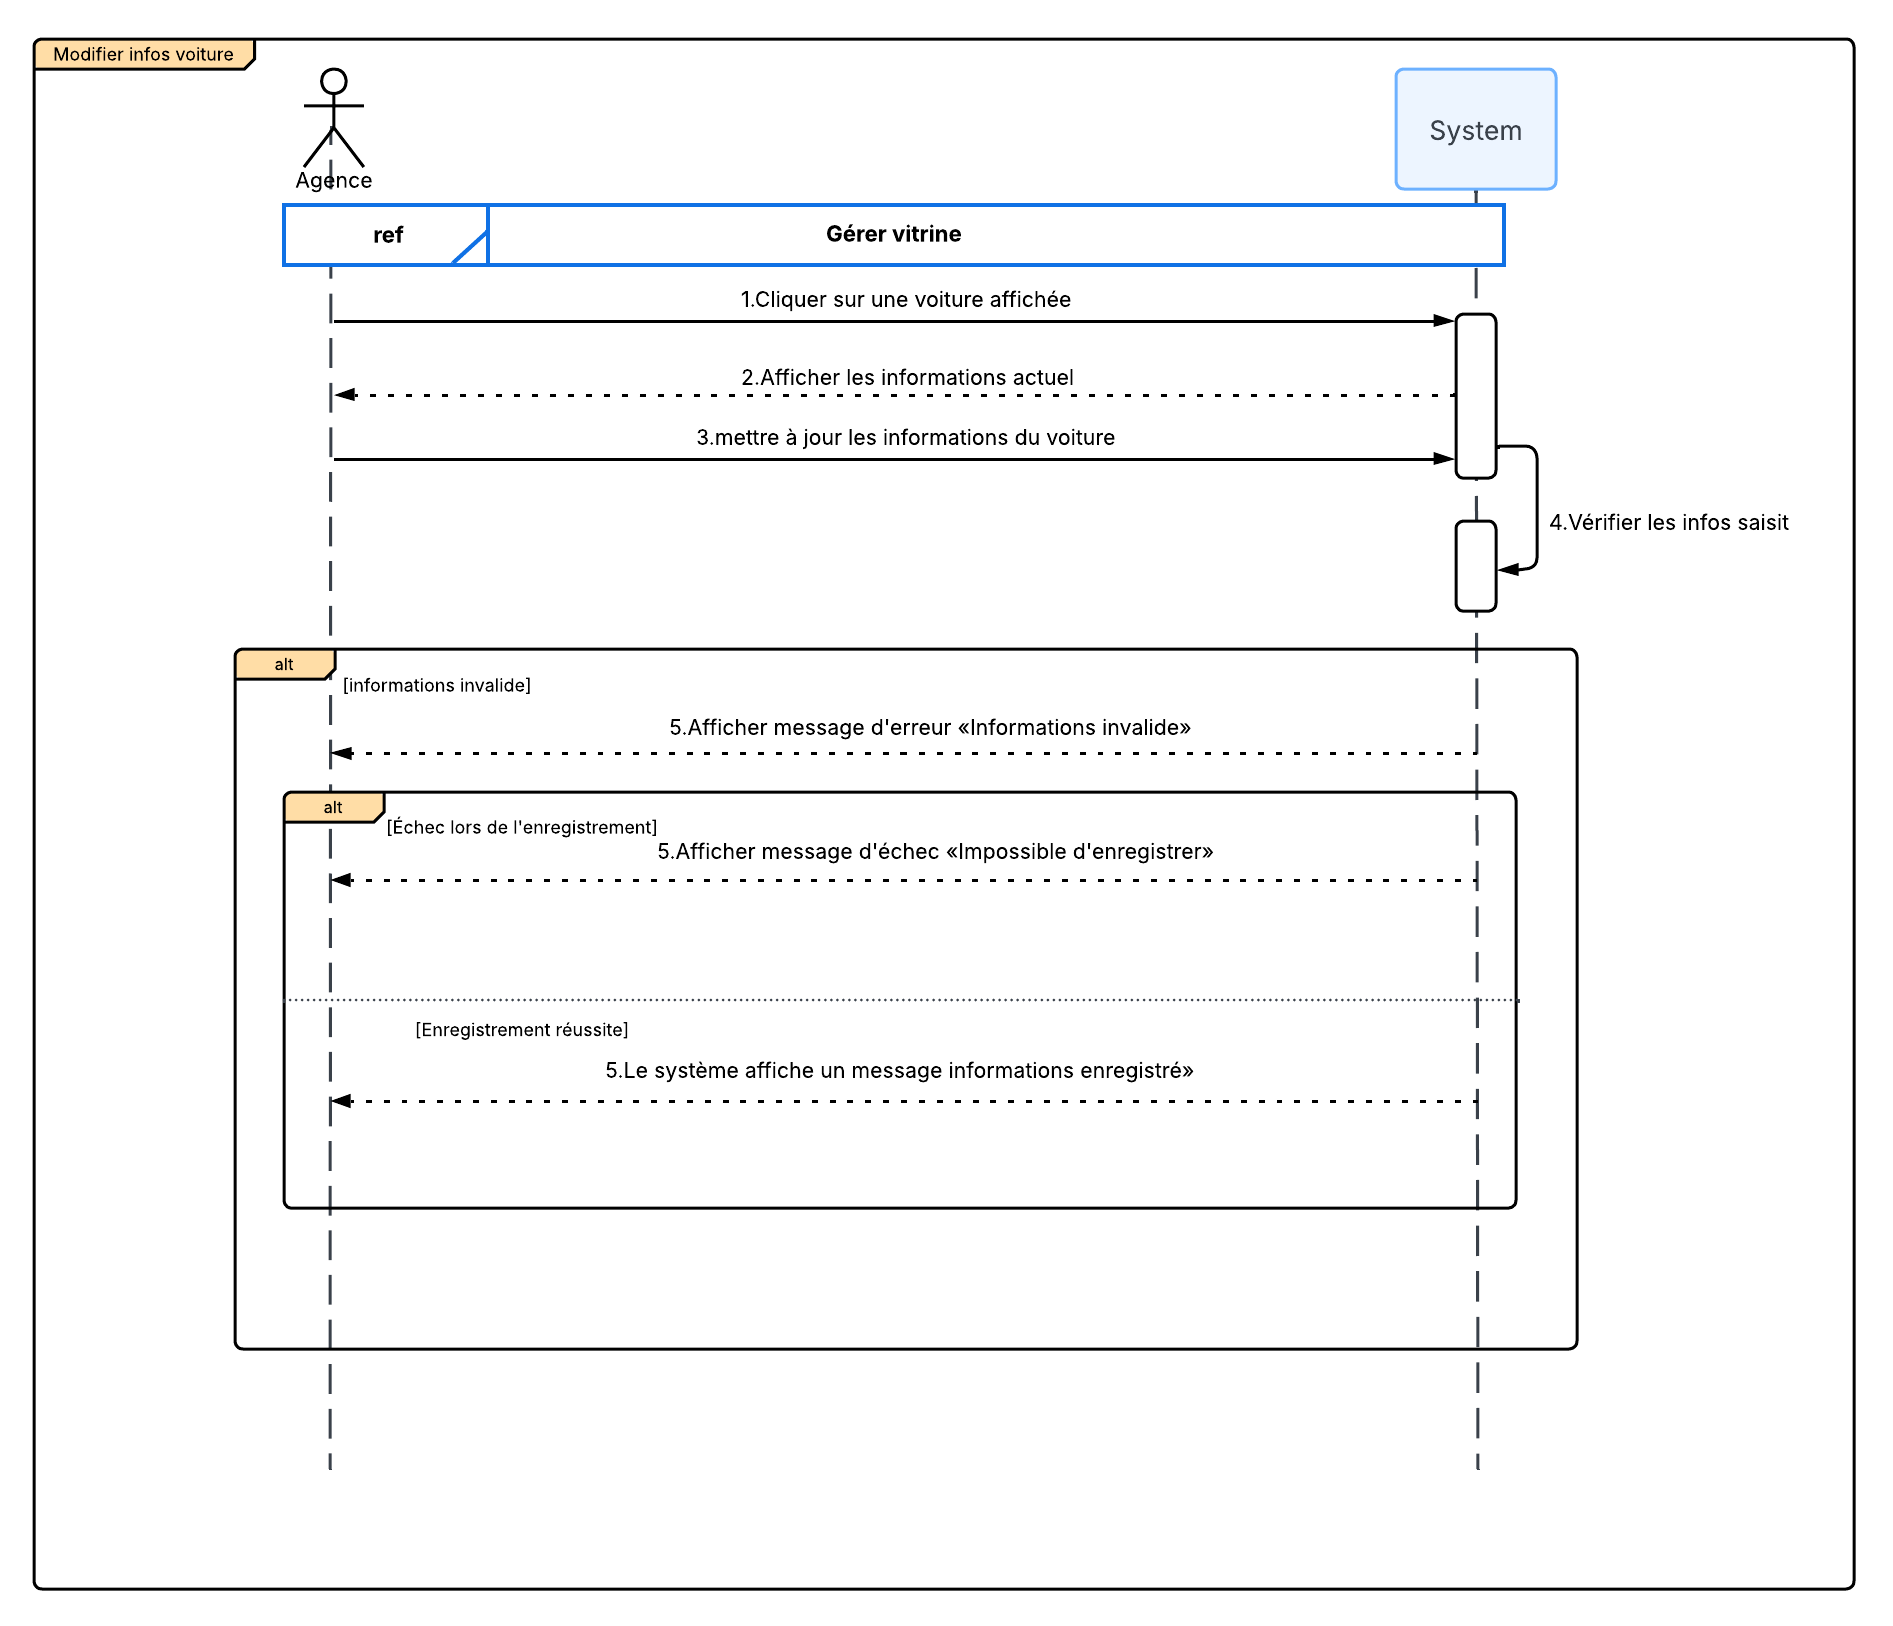
\includegraphics[width=1\textwidth]{Chapitres/Figures/Diag_seq_modifier_infos_voiture.png}
    \caption{Diagramme de séquence système de cas d'utilisation «Modifier infos voiture»}
    \label{fig:modifier_infos_voiture}
\end{figure}
%%%%%%%%%%%%%%%%%%
\subsection{Analyse de cas d'utilisation «Ajouter voiture»}
\label{sec:ajouter_voiture}
Dans la suite, nous présentons unee description textuelle accompagnée d'une diagramme 
de séquence du cas d'utilisation \textbf{«Ajouter voiture»} de l'acteur 
\textit{Agence}.

\begin{table}[H]
\centering
\caption{Description textuelle du cas d'utilisation «Ajouter voiture»}
\label{tab:ajouter_voiture}
\renewcommand{\arraystretch}{1.3}
\resizebox{\textwidth}{!}{%
\begin{tabular}{|l|p{11cm}|}
\hline
\textbf{Élément} & \textbf{Description} \\
\hline
Nom & Ajouter voiture \\
\hline
Acteur & Agence \\
\hline
Description brève & Permet à l'agence d'ajouter une voiture. \\
\hline
Précondition & 
 L'agence est authentifié. \newline
 Le système est accessible. \\
\hline
Postcondition & 
 Une voiture est ajoutée. \\
\hline
Enchaînement principal & 
1. L'agence accède à la page «Vitrine». \newline
2. Le système affiche la liste des voitures. \newline
3. L'agence choisit d'ajouter une voiture. \newline
4. L'agence saisit les informations nécessaires. \newline
5. Le système vérifie les données. \newline
6. Le système enregistre l'voiture. \newline
7. Le système affiche une message de confirmation. \\
\hline
\multirow{6}{*}{\textbf{Scénario alternatif}} & 5.1 Informations invalides.\\
& \quad 5.1.1 Le système affiche une message d'erreur. \\
& 6.1 Erreur lors de l'enregistrement. \\
& \quad 6.1.1 Le système affiche une message d'échec. \\
\hline
\end{tabular}%
}
\end{table}

\begin{figure}[H]
    \centering
    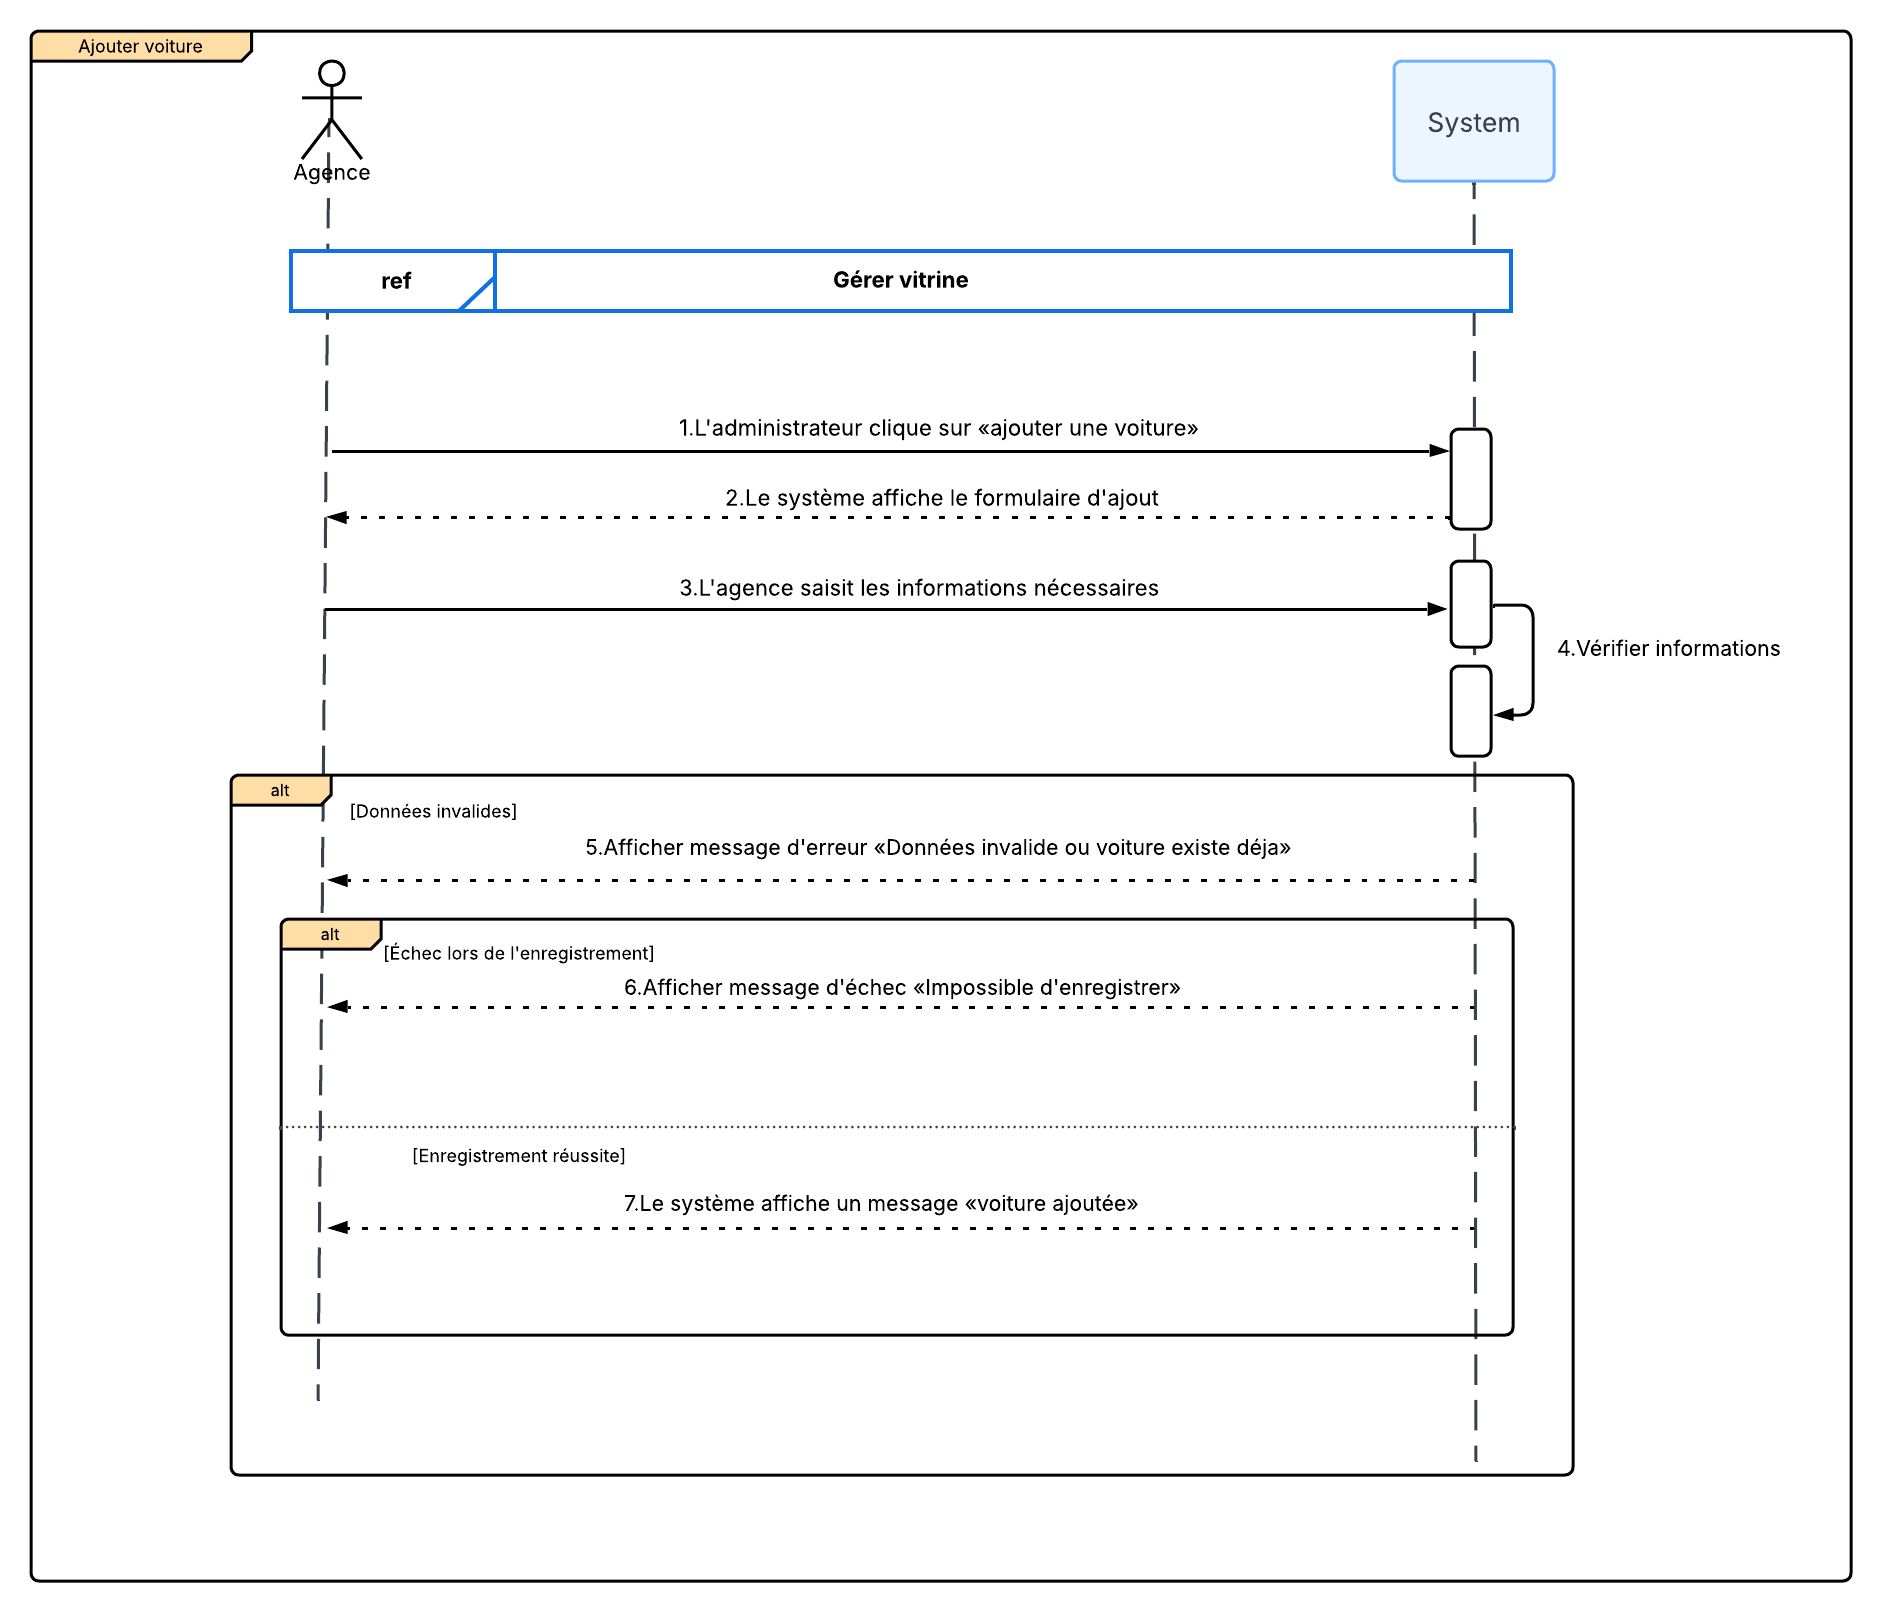
\includegraphics[width=1\textwidth]{Chapitres/Figures/Diag_seq_ajouter_voiture.png}
    \caption{Diagramme de séquence système de cas d'utilisation «Ajouter voiture»}
    \label{fig:ajouter_voiture}
\end{figure}


%%%%%%%%%%%%%%%%%%%%%%%%%%%%%%%%%%%%%%%%%%%%%%%%%%%%%%%%%%%%%%%%%%%%%%%%%%%


%%%%%%%%%%%%%%%%%%%%%%%%%
\FloatBarrier
\section{Conception des cas d'utilisation}
\label{conception_des_cas_d_utilisation}
Nous illustrerons dans cette section la conception de ce premier sprint à travers la
réalisation d'un diagramme des classes pour chaque module, ainsi que d'un diagramme
de séquence détaillé correspondant à chaque cas d'utilisation analysé
%%%%%%%%%%%%%%%%%%%%%%%%%%%%%%%%%%%%%%%%%%%%%%%%%%%%%%%%%%%%%%%%%%%%%%%%%%%
\newpage
\subsection{Diagramme des classes participantes}
\label{Diag_classes_participantes_s1}

Un diagramme des classes participantes est une représentation UML utilisée 
dans la phase d’analyse pour décrire la réalisation d’un cas d’utilisation 
spécifique. Il met en évidence les différentes classes impliquées dans 
l’interaction, ainsi que leurs responsabilités et leurs relations, afin de 
structurer le comportement du système selon une approche orientée objet.\cite{stackoverflow}

Ce diagramme repose généralement sur trois catégories principales de classes d’analyse :

\begin{enumerate}
    \item \textbf{Les classes frontières (ou classes de dialogue)} : 
    Elles assurent l’interaction entre l’utilisateur et le système. 
    Elles contiennent des attributs correspondant aux données affichées ou saisies 
    (champs de formulaires, résultats, etc.) et des opérations représentant 
    les actions effectuées par l’utilisateur via l’interface homme-machine (IHM).\cite{stackoverflow}

    \item \textbf{Les classes de contrôle} : 
    Elles orchestrent le déroulement du cas d’utilisation. 
    Elles implémentent la logique applicative, coordonnent les échanges entre 
    les classes frontières et les classes entités, et encapsulent les règles 
    métier ainsi que les traitements du système.\cite{stackoverflow}

    \item \textbf{Les classes entités} : 
    Elles représentent les données métier du système. 
    Ces classes contiennent des attributs persistants correspondant aux informations 
    stockées (par exemple dans une base de données) et peuvent inclure des opérations 
    liées à la gestion de ces données.\cite{stackoverflow}
\end{enumerate}

\subsubsection{Diagramme des classes participantes par acteur «Internaute»}
\label{Diag_classes_participantes_internaute_s1}
\begin{figure}[H]
    \centering
    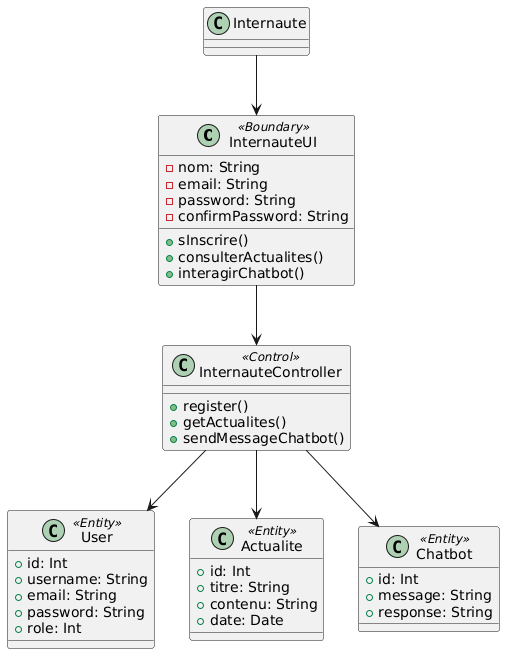
\includegraphics[width=1\textwidth]{Chapitres/Figures/classes_participantes__internaute_s1.png}
    \caption{Diagramme des classes participantes par acteur Internaute}
    \label{fig:classes_participantes_internaute_s1}
\end{figure}

\subsubsection{Diagramme des classes participantes par acteur «Utilisateur»}
\label{Diag_classes_participantes_utilisateur_s1}
\begin{figure}[H]
    \centering
    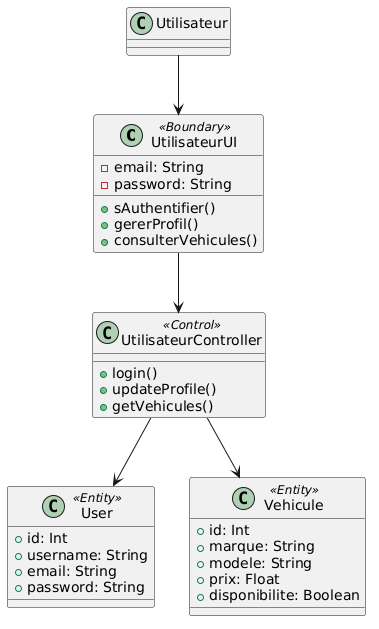
\includegraphics[width=1\textwidth]{Chapitres/Figures/classes_participantes__utilisateur_s1.png}
    \caption{Diagramme des classes participantes par acteur Utilisateur}
    \label{fig:classes_participantes_utilisateur_s1}
\end{figure}

\subsubsection{Diagramme des classes participantes par acteur «Agence»}
\label{Diag_classes_participantes_agence_s1}
\begin{figure}[H]
    \centering
    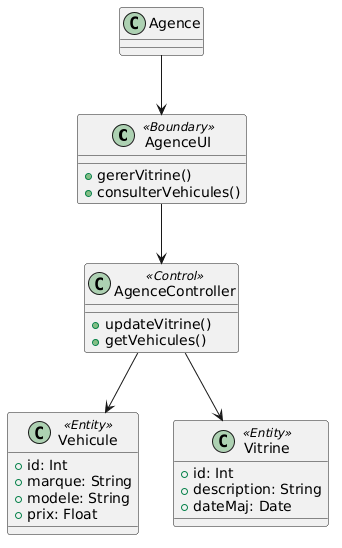
\includegraphics[width=1\textwidth]{Chapitres/Figures/classes_participantes__agence_s1.png}
    \caption{Diagramme des classes participantes par acteur Agence}
    \label{fig:classes_participantes_agence_s1}
\end{figure}

\subsubsection{Diagramme des classes participantes par acteur «Administrateur»}
\label{Diag_classes_participantes_administrateur_s1}
\begin{figure}[H]
    \centering
    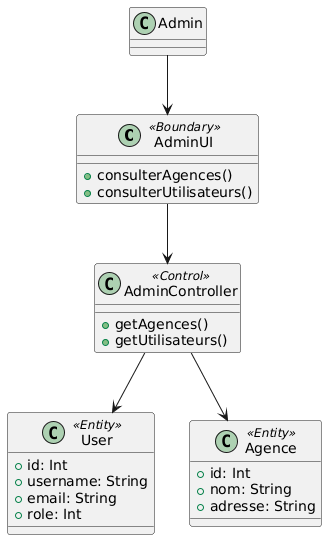
\includegraphics[width=1\textwidth]{Chapitres/Figures/classes_participantes__admin_s1.png}
    \caption{Diagramme des classes participantes par acteur Administrateur}
    \label{fig:classes_participantes_admin_s1}
\end{figure}

%%%%%%%%%%%seq_détaillé%%%%%%%%%%%%%%%%%%%%%%%%%%%%%%%%%%%%%%%%%%%%%%%%%%%%%%%%%%%%%%%%%%%%%%%%%%%%%%%%%%%%%
\section{Diagrammes de séquence détaillés du premier sprint}
\label{sec:diag_seq_detail_s1}
\textit{"Les diagrammes de séquence sont un outil essentiel en génie logiciel pour visualiser les interactions entre les objets d’un système au fil du temps. Ils aident à comprendre le comportement dynamique d’un système, à concevoir son architecture et à documenter des processus complexes. Ce guide couvrira les concepts clés, les recommandations, un exemple concret et une étude de cas pour vous aider à maîtriser les diagrammes de séquence.''}\cite{cybermedian}


%====================================================x²
\subsection{Diagrammes de séquence détaillés de l’acteur Internaute}
\label{sec:diag_seq_internaute}

\subsubsection{Diagrammes de séquence détaillé du cas d’utilisation « Consulter actualités »}
\label{sec:diag_seq_det_consulter_actualite}
\begin{figure}[H]
    \centering
    
\includegraphics[width=0.8\textwidth]{Chapitres/figures/diag_seq_det/seq_det_s1/seq_det_consulter_actualite.png}
    \caption{Diagramme de séquence détaillé du cas d’utilisation « Consulter actualités »}
    \label{fig:seq_det_consulter_actualite}
\end{figure}

\subsubsection{Diagrammes de séquence détaillé du cas d’utilisation « S’inscrire »}
\label{sec:diag_seq_det_s_inscrire}
\begin{figure}[H]
    \centering
    
\includegraphics[width=0.95\textwidth]{Chapitres/figures/diag_seq_det/seq_det_s1/seq_det_s_inscrire.png}
    \caption{Diagramme de séquence détaillé du cas d’utilisation « S’inscrire »}
    \label{fig:seq_det_s_inscrire}
\end{figure}

%====================================================
\subsection{Diagrammes de séquence détaillés de l’acteur Utilisateur}
\label{sec:diag_seq_utilisateur}


\subsubsection{Diagrammes de séquence détaillé du cas d’utilisation « S’authentifier »}
\label{sec:diag_seq_det_s_authentifier}
\begin{figure}[H]
    \centering
    
\includegraphics[width=0.85\textwidth]{Chapitres/figures/diag_seq_det/seq_det_s1/seq_det_s_authentifier.png}
    \caption{Diagramme de séquence détaillé du cas d’utilisation « S’authentifier »}
    \label{fig:seq_det_s_authentifier}
\end{figure}


\subsubsection{Diagrammes de séquence détaillé du cas d’utilisation « Interagir avec Chatbot »}
\label{sec:diag_seq_det_chatbot}
\begin{figure}[H]
    \centering
    
\includegraphics[width=0.85\textwidth]{Chapitres/figures/diag_seq_det/seq_det_s1/seq_det_chatbot.png}
    \caption{Diagramme de séquence détaillé du cas d’utilisation « Interagir avec Chatbot »}
    \label{fig:seq_det_chatbot}
\end{figure}

\subsubsection{Diagrammes de séquence détaillé du cas d’utilisation « Consulter profil »}
\label{sec:diag_seq_det_consulter_profil}
\begin{figure}[H]
    \centering
    
\includegraphics[width=0.85\textwidth]{Chapitres/figures/diag_seq_det/seq_det_s1/seq_det_consulter_profil.png}
    \caption{Diagramme de séquence détaillé du cas d’utilisation « Consulter profil »}
    \label{fig:seq_det_consulter_profil}
\end{figure}

%====================================================
\subsection{Diagrammes de séquence détaillés de l’acteur Administrateur}
\label{sec:diag_seq_admin_s1}

\subsubsection{Diagrammes de séquence détaillé du cas d’utilisation « Ajouter agence »}
\label{sec:diag_seq_det_ajouter_agence}
\begin{figure}[H]
    \centering
    
\includegraphics[width=0.8\textwidth]{Chapitres/figures/diag_seq_det/seq_det_s1/seq_det_ajouter_agence.png}
    \caption{Diagramme de séquence détaillé du cas d’utilisation « Ajouter agence »}
    \label{fig:seq_det_ajouter_agence}
\end{figure}

\subsubsection{Diagrammes de séquence détaillé du cas d’utilisation « Bloquer/Débloquer agence »}
\label{sec:sec_diag_seq_det_bloquer_agence}
\begin{figure}[H]
    \centering
    
\includegraphics[width=0.8\textwidth]{Chapitres/figures/diag_seq_det/seq_det_s1/seq_det_bloquer_agence.png}
    \caption{Diagramme de séquence détaillé du cas d’utilisation « Bloquer/Débloquer agence »}
    \label{fig:seq_det_bloquer_agence}
\end{figure}

\subsubsection{Diagrammes de séquence détaillé du cas d’utilisation « Ajouter utilisateur »}
\label{sec:diag_seq_det_ajouter_utilisateur}
\begin{figure}[H]
    \centering
    
\includegraphics[width=0.8\textwidth]{Chapitres/figures/diag_seq_det/seq_det_s1/seq_det_ajouter_utilisateur.png}
    \caption{Diagramme de séquence détaillé du cas d’utilisation « Ajouter utilisateur »}
    \label{fig:seq_det_ajouter_utilisateur}
\end{figure}

\subsubsection{Diagrammes de séquence détaillé du cas d’utilisation « Bloquer/Débloquer utilisateur »}
\label{sec:diag_seq_det_bloquer_agence}
\begin{figure}[H]
    \centering
    
\includegraphics[width=0.8\textwidth]{Chapitres/figures/diag_seq_det/seq_det_s1/seq_det_bloquer_utilisateur.png}
    \caption{Diagramme de séquence détaillé du cas d’utilisation « Bloquer/Débloquer utilisateur »}
    \label{fig:seq_det_bloquer_utilisateur}
\end{figure}

\newpage
\FloatBarrier
\section{Diagramme de classe du premier sprint}
\label{section3.diag_classes}
Un diagramme de classes est une représentation graphique qui identifie les principales classes d’un système, leurs attributs, leurs méthodes et les relations qui les lient. Chaque classe est figurée par un rectangle divisé en trois parties (nom, attributs, opérations), et les liens entre classes traduisent des relations comme l’héritage, l’association ou la dépendance. Ce type de diagramme permet de structurer et de visualiser l’architecture logicielle, en offrant une vue claire des entités et de leurs interactions essentielles.\cite{Lucidchart}
%%%%%%%%%%%%%%%%%%%%%%%%%%%%%%%%%%%%%%%%%%%%%%%%%%%%%%%%%%%%%%%%%%%%%%%%%%%

\begin{figure}[H]
    \centering
    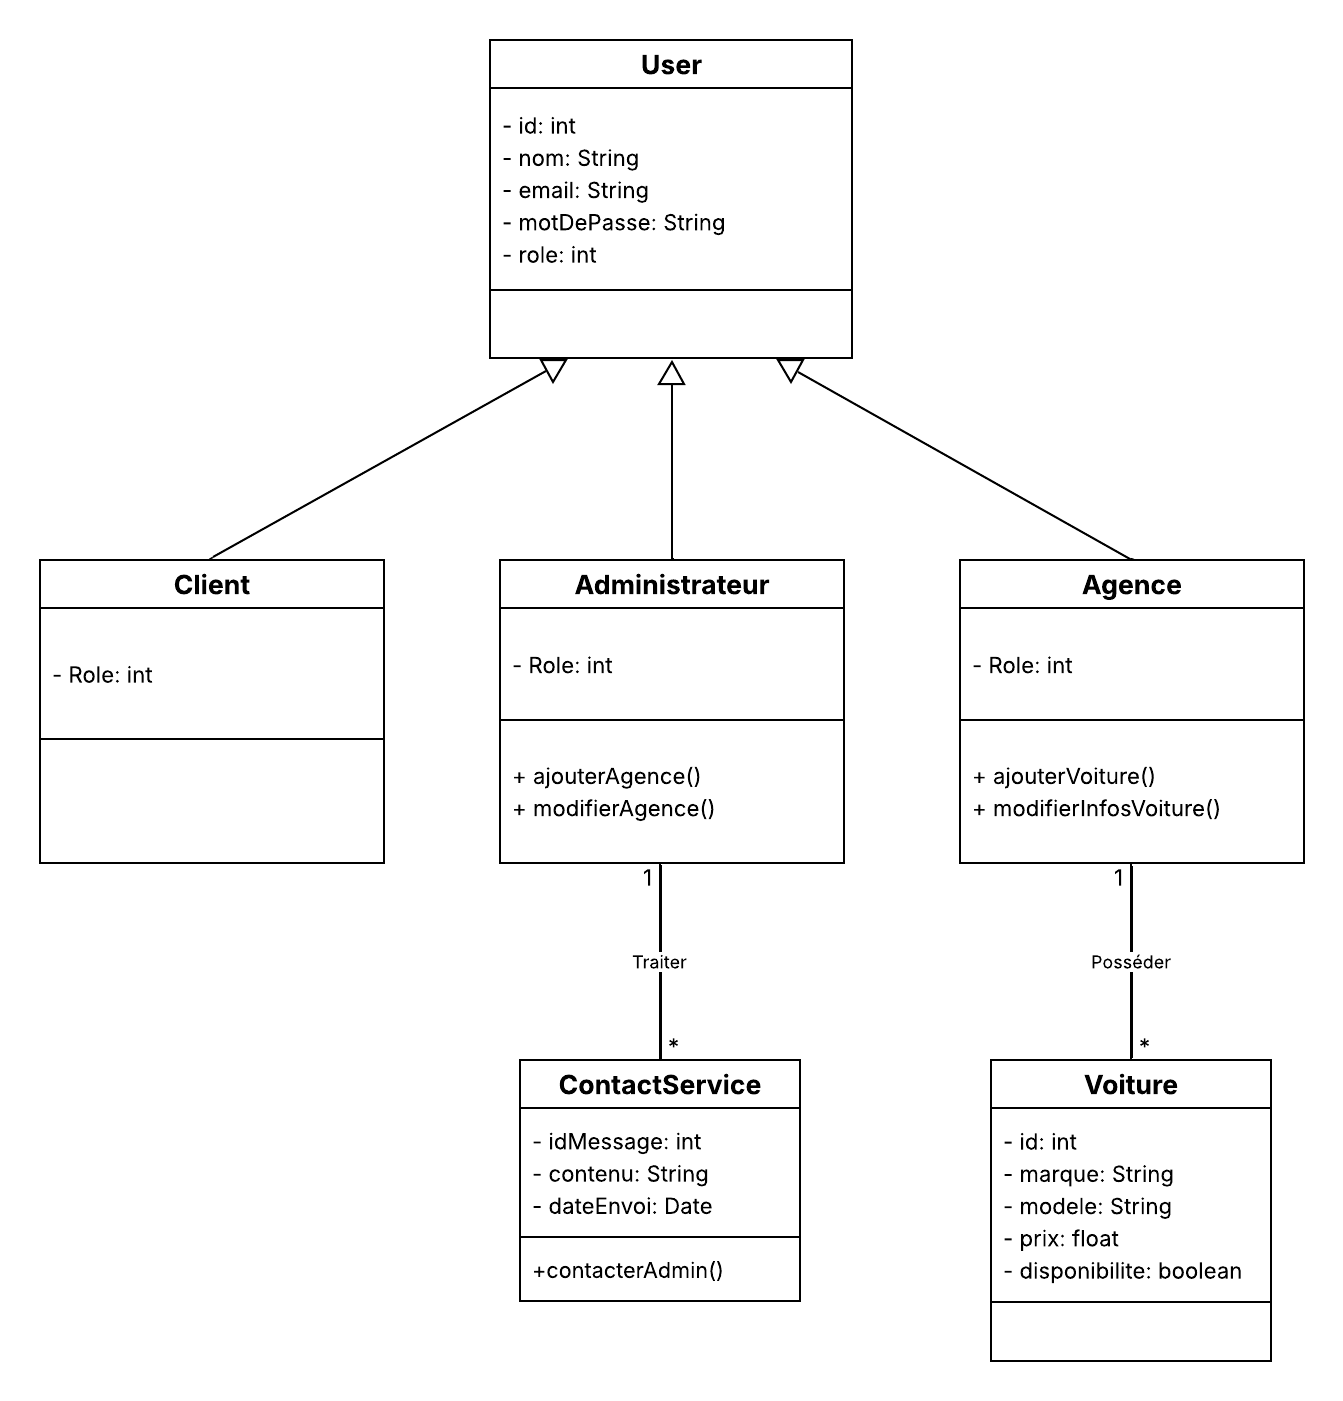
\includegraphics[width=1\textwidth]{Chapitres/Figures/Diag_classe_sprint_1.png}
    \caption{Diagramme de classe du premier sprint}
    \label{fig:diag_classes}
\end{figure}
%%%%%%%%%%%%%%%%%%%%%%%%%%%%%%%%%%%%%%%%%%%%%%%%%%%%%%%%%%%%%%%%%%%%%%%%%%%%%%%%%%%%%%%%%%%%%%%%%%%%%%%%%%%%
\section{Implémentation}
\label{sec:implementation_s1}

Le module d'implémentation d'un projet prévoit l'implémentation des fonctions qui ont été réalisées au cours du premier sprint.

\subsection{Tables de la base de données}

Le tableau ci-joint décrit le répertoire de données afin d'illustrer les attributs que l'on retrouve dans les différentes classes, ainsi que leurs étiquettes et leurs types.

\subsubsection{Tableau « users »}

\begin{table}[H]
\centering
\caption{Tableau « users »}
\label{tab:users}
\renewcommand{\arraystretch}{1.3}
\resizebox{\textwidth}{!}{%
\begin{tabular}{|l|l|p{4cm}|l|}
\hline
\textbf{Champs} & \textbf{Type} & \textbf{Libellé} & \textbf{Contraintes} \\
\hline
id & Int & Identifiant unique de l'utilisateur & PRIMARY KEY, NOT NULL \\
\hline
name & String & Le nom de l'utilisateur & NOT NULL \\
\hline
email & String & L'email de l'utilisateur & NOT NULL, UNIQUE \\
\hline
email\_verified\_at & Timestamp & La date de vérification de l'email & NULLABLE \\
\hline
password & String & Le mot de passe de l'utilisateur & NOT NULL \\
\hline
must\_change\_password & Tinyint(1) & Indique si l'utilisateur doit changer son mot de passe & NOT NULL, DEFAULT 0 \\
\hline
role & Enum & Le rôle de l'utilisateur (client / agency\_admin / super\_admin) & NOT NULL \\
\hline
agency\_id & BigInt & Identifiant unique de l'agence & FOREIGN KEY, NULLABLE \\
\hline
phone & String & Le numéro de téléphone de l'utilisateur & NULLABLE \\
\hline
address & Text & L'adresse de l'utilisateur & NULLABLE \\
\hline
driver\_license & String & Le permis de conduire de l'utilisateur & NULLABLE \\
\hline
is\_suspended & Boolean & Indique si l'utilisateur est suspendu & NOT NULL, DEFAULT 0 \\
\hline
suspension\_reason & Text & La raison de la suspension de l'utilisateur & NULLABLE \\
\hline
suspended\_at & Timestamp & La date de suspension de l'utilisateur & NULLABLE \\
\hline
remember\_token & String & Token de mémorisation & NULLABLE \\
\hline
created\_at & Timestamp & Date de création & NOT NULL \\
\hline
updated\_at & Timestamp & Date de modification & NOT NULL \\
\hline
\end{tabular}%
}
\end{table}

\subsubsection{Tableau « vehicles »}

\begin{table}[H]
\centering
\caption{Tableau « vehicles »}
\label{tab:vehicles}
\renewcommand{\arraystretch}{1.3}
\resizebox{\textwidth}{!}{%
\begin{tabular}{|l|l|p{4cm}|l|}
\hline
\textbf{Champs} & \textbf{Type} & \textbf{Libellé} & \textbf{Contraintes} \\
\hline
id & Int & Identifiant unique du véhicule & PRIMARY KEY, NOT NULL \\
\hline
brand & String & La marque du véhicule & NOT NULL \\
\hline
model & String & Le modèle du véhicule & NOT NULL \\
\hline
year & Int & L'année du véhicule & NOT NULL \\
\hline
mileage & Int & Le kilométrage du véhicule & NOT NULL \\
\hline
daily\_price & Decimal(8,2) & Le prix journalier de location & NOT NULL \\
\hline
caution\_amount & Decimal(10,2) & Le montant de la caution fixé par l'agence & NULLABLE \\
\hline
license\_plate & String & La plaque d'immatriculation & NOT NULL, UNIQUE \\
\hline
color & String & La couleur du véhicule & NOT NULL \\
\hline
seats & Int & Le nombre de places & NOT NULL \\
\hline
transmission & Enum & Le type de transmission (manual / automatic) & NOT NULL \\
\hline
fuel\_type & Enum & Le type de carburant (petrol / diesel / electric / hybrid) & NOT NULL \\
\hline
status & Enum & L'état du véhicule (available / reserved / in\_use / returned) & NOT NULL, DEFAULT available \\
\hline
agency\_id & BigInt UNSIGNED & Identifiant unique de l'agence & FOREIGN KEY, NOT NULL \\
\hline
created\_at & Timestamp & Date de création & NULLABLE \\
\hline
updated\_at & Timestamp & Date de modification & NULLABLE \\
\hline
images & Text & Les images du véhicule & NULLABLE \\
\hline
\end{tabular}%
}
\end{table}

\subsection{Réalisation des interfaces du premier sprint}

Nous présentons dans cette section les interfaces graphiques développées lors du premier sprint.

\subsubsection{Interface d'inscription :}

\begin{figure}[H]
    \centering
    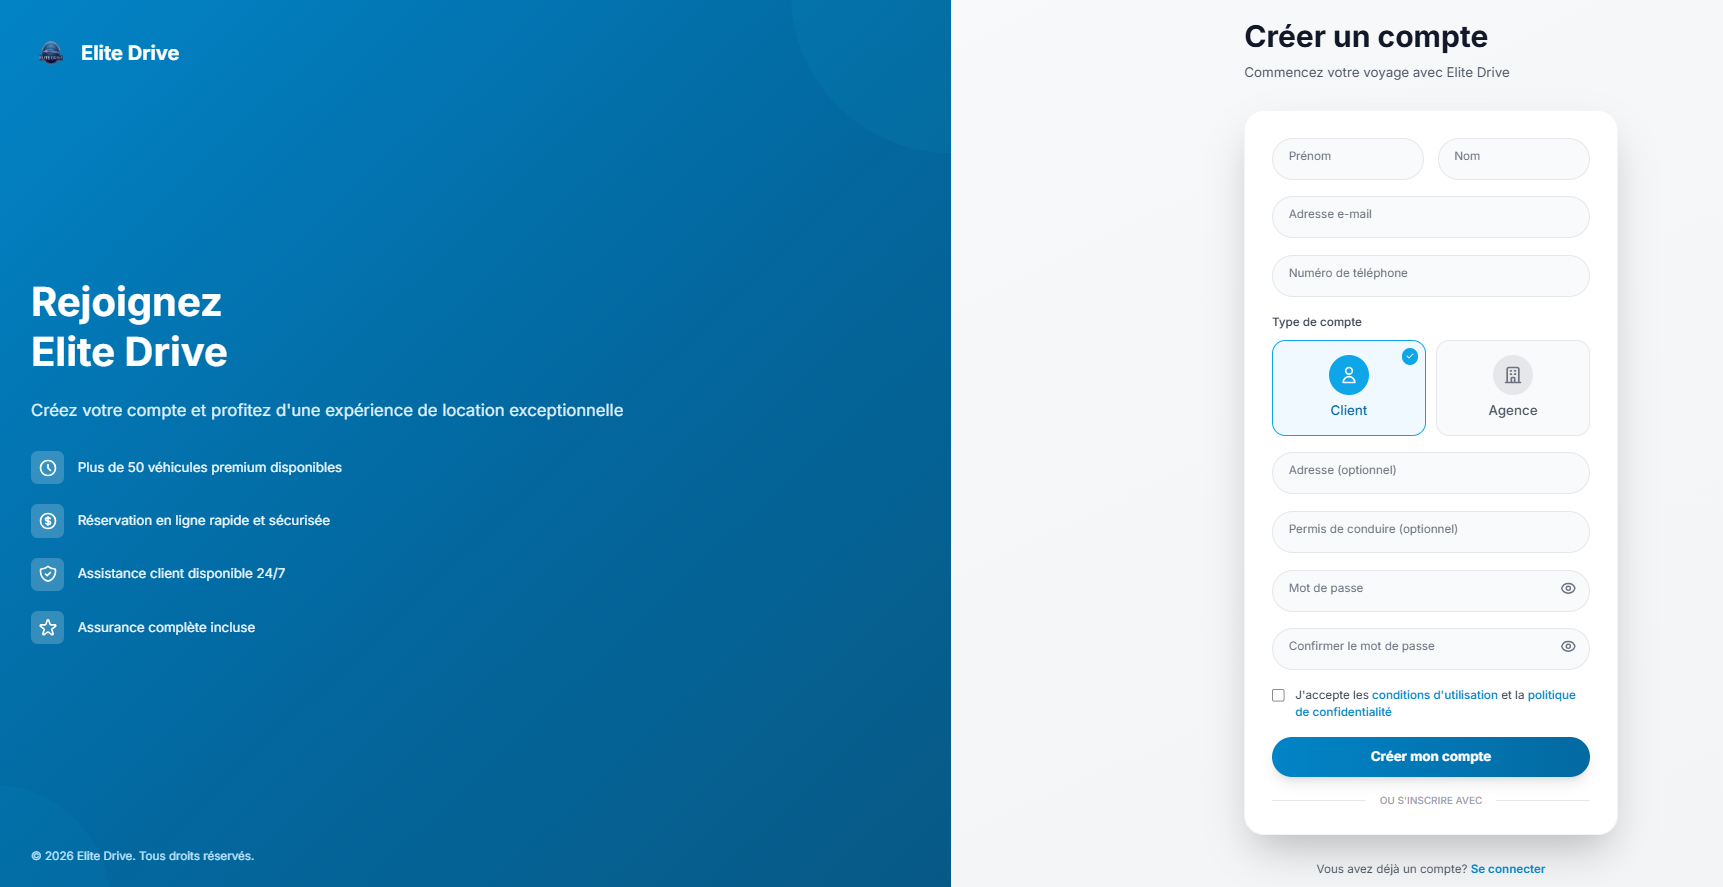
\includegraphics[width=0.9\linewidth]{Chapitres/Figures/inter_inscrire.png}
    \caption{Interface d'inscription}
    \label{fig:interface_inscription_s1}
\end{figure}

\subsubsection{Interface d'authentication :}

\begin{figure}[H]
    \centering
    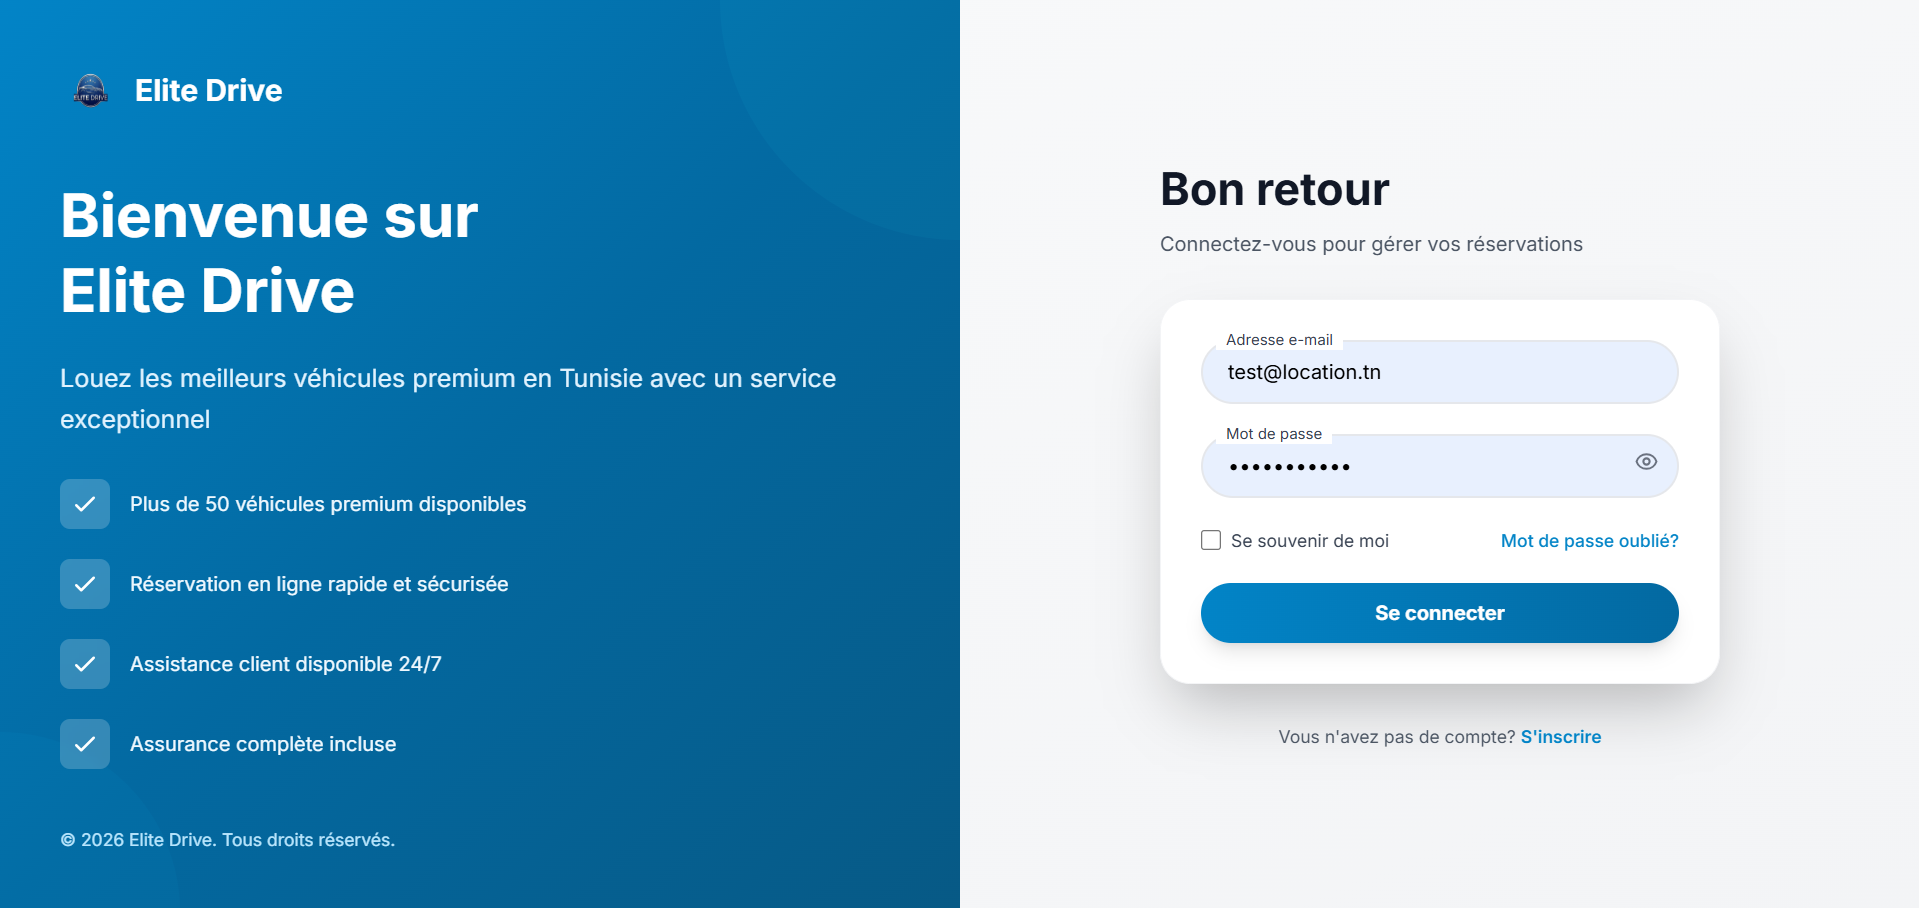
\includegraphics[width=0.9\linewidth]{Chapitres/Figures/inter_auth.png}
    \caption{Interface d'authentification}
    \label{fig:interface_authentification_s1}
\end{figure}

\subsubsection{Interface profil :}

\begin{figure}[H]
    \centering
    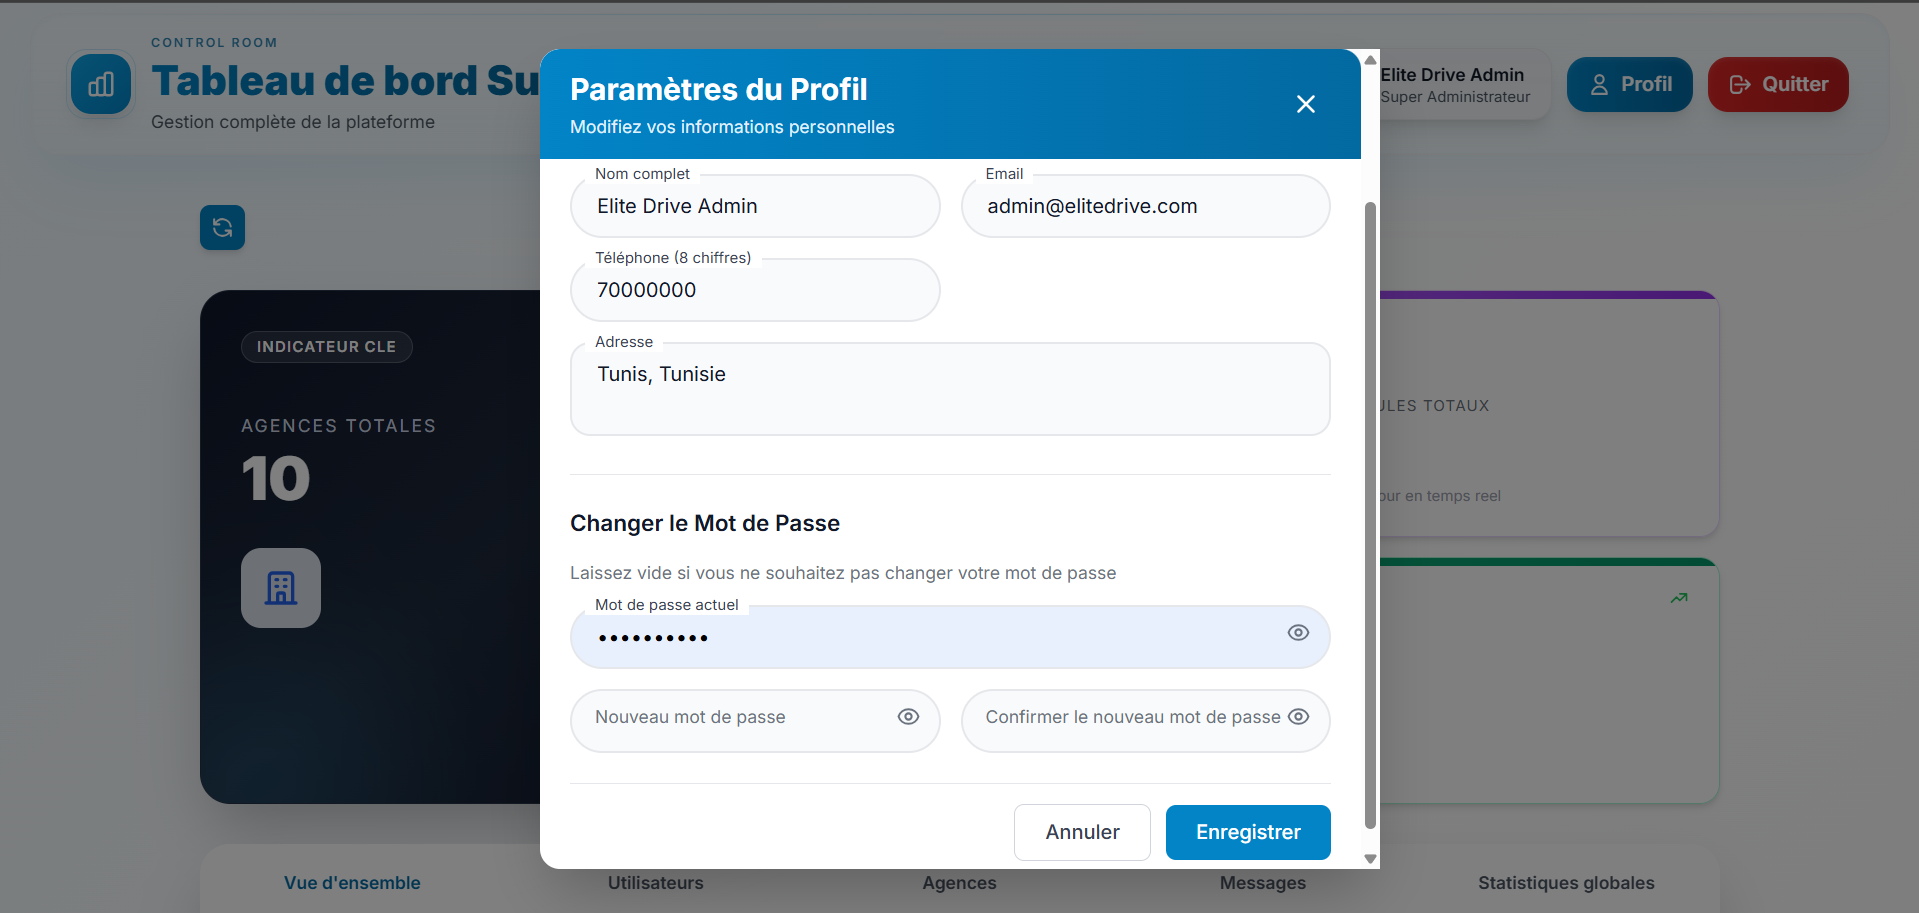
\includegraphics[width=0.9\linewidth]{Chapitres/Figures/inter_profil.png}
    \caption{Interface profil}
    \label{fig:interface_profil_s1}
\end{figure}

\subsubsection{Interface chatbot :}

\begin{figure}[H]
    \centering
    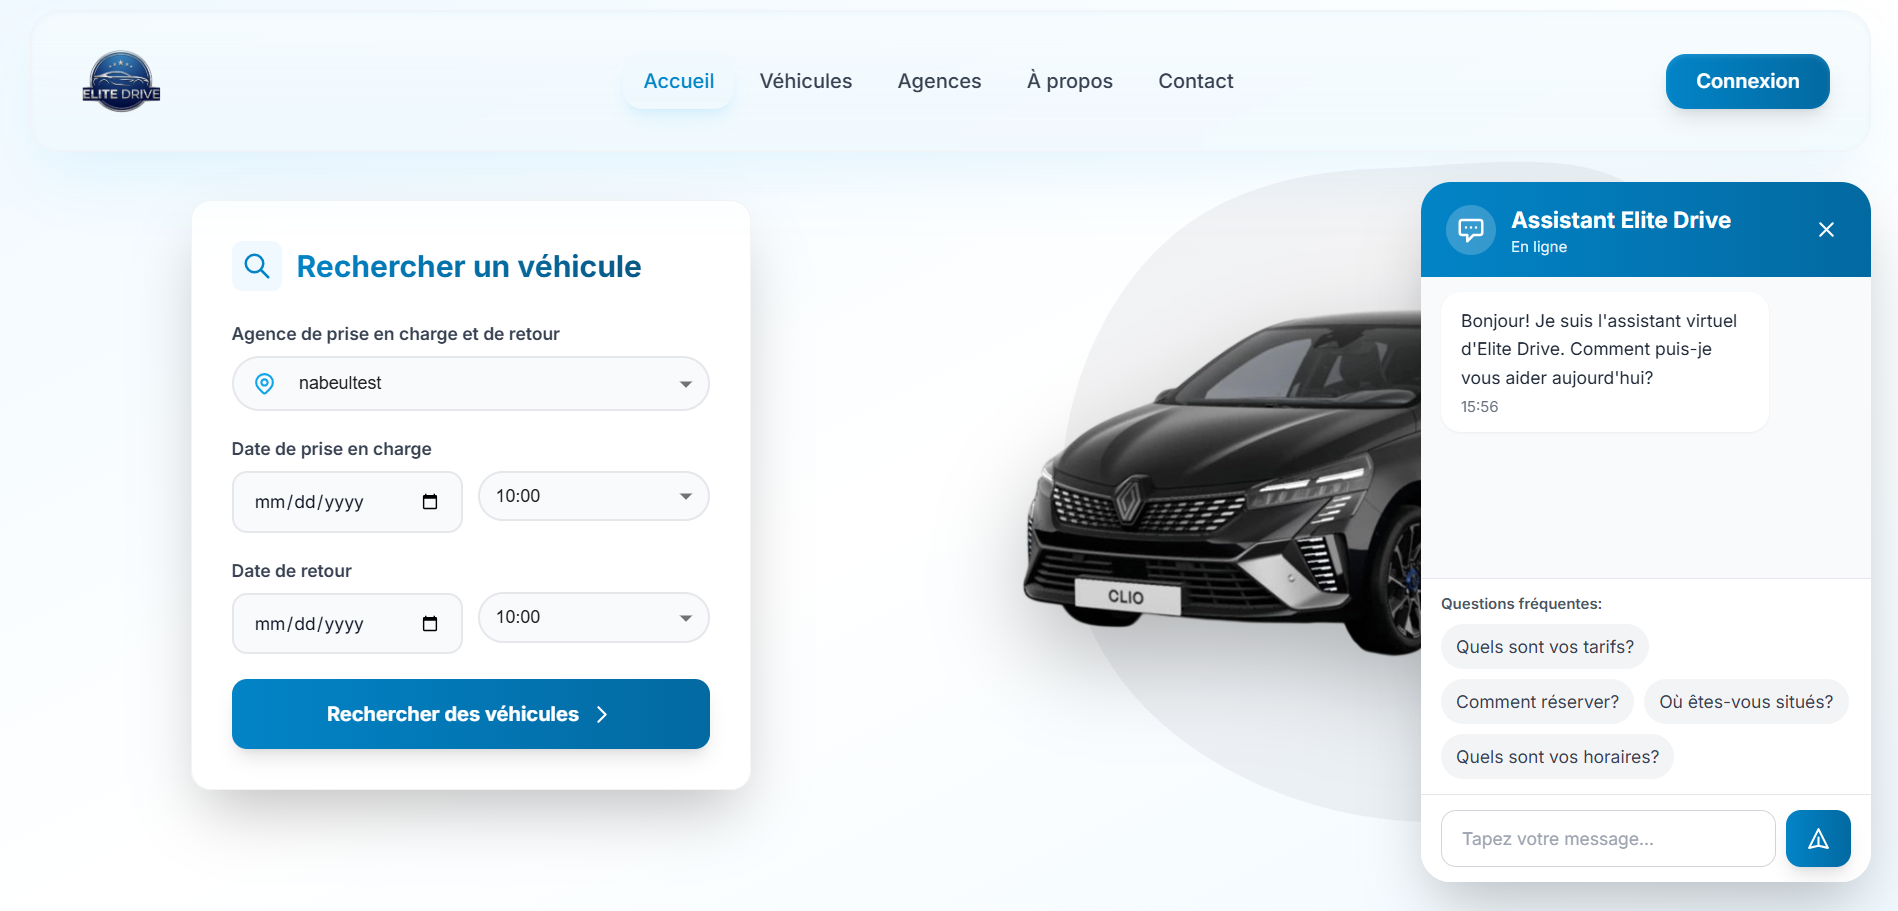
\includegraphics[width=0.9\linewidth]{Chapitres/Figures/inter_chatbot.png}
    \caption{Interface chatbot}
    \label{fig:interface_chatbot_s1}
\end{figure}

\subsubsection{Interface vitrine :}

\begin{figure}[H]
    \centering
    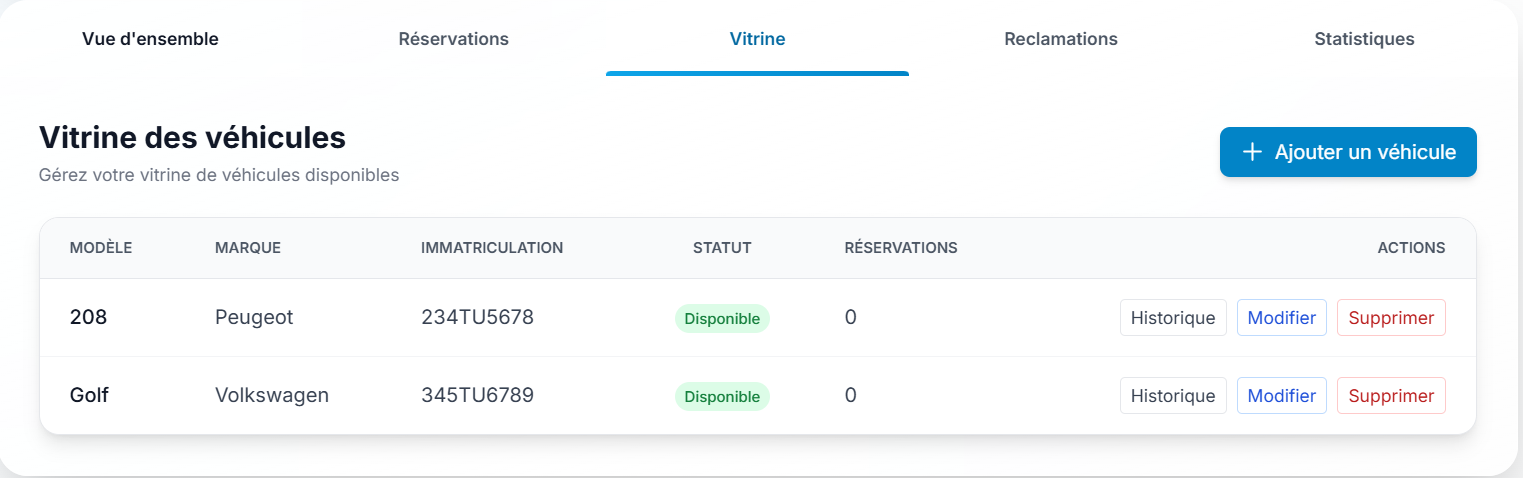
\includegraphics[width=0.9\linewidth]{Chapitres/Figures/inter_vitrine.png}
    \caption{Interface vitrine}
    \label{fig:interface_vitrine_s1}
\end{figure}

\subsubsection{Interface bloquer/debloquer une agence :}

\begin{figure}[H]
    \centering
    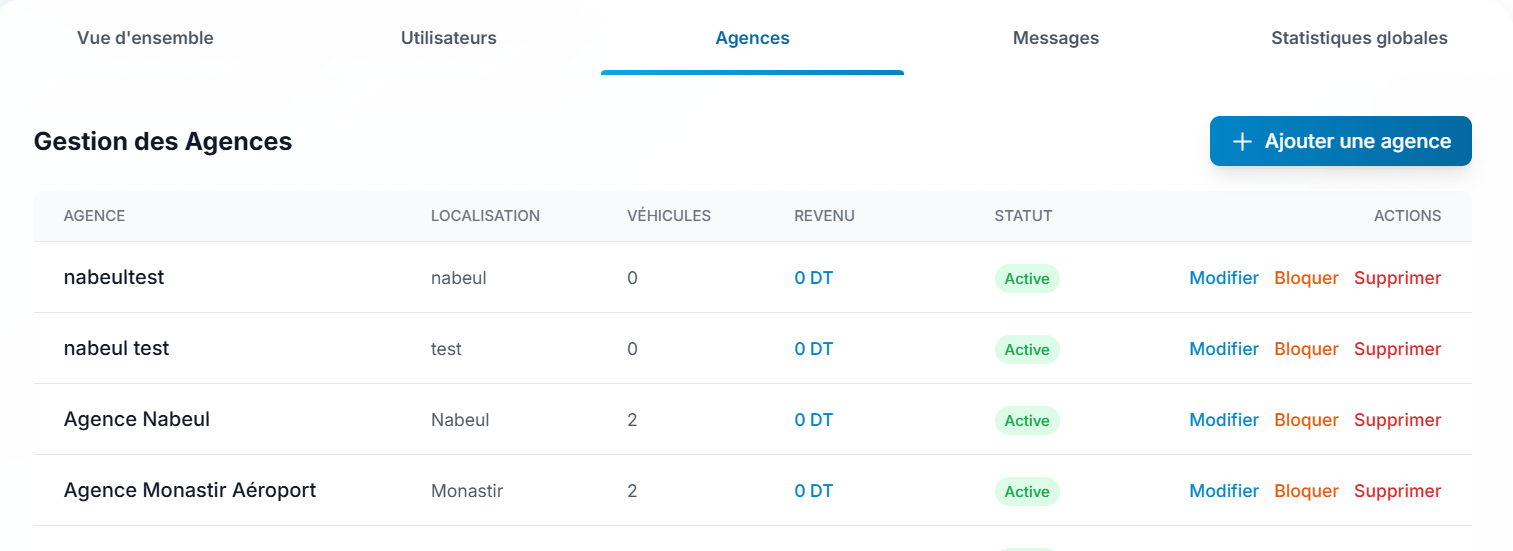
\includegraphics[width=0.9\linewidth]{Chapitres/Figures/inter_bloqAgence.png}
    \caption{Interface bloquer/débloquer une agence}
    \label{fig:interface_bloquer_debloquer_agence_s1}
\end{figure}

%%%%%%%%%%%%%%%%%%%%%%%%%%%%%%%%%%%%%%%%%%%%%%%%%%%%%%%%%%%%%%%%%%%%%%%%%%%%%%%%%%%%%%%%%%%%%%%%%%%%%%%%%%%%
\section{Test unitaire}
\subsection{Test unitaire du cas d’utilisation «S’authentifier»}

Cette section se concentre sur la récupération du code pour le cas «S’authentifier».

\subsection*{— Code source de la méthode d’authentification :}

\begin{figure}[H]
    \centering
    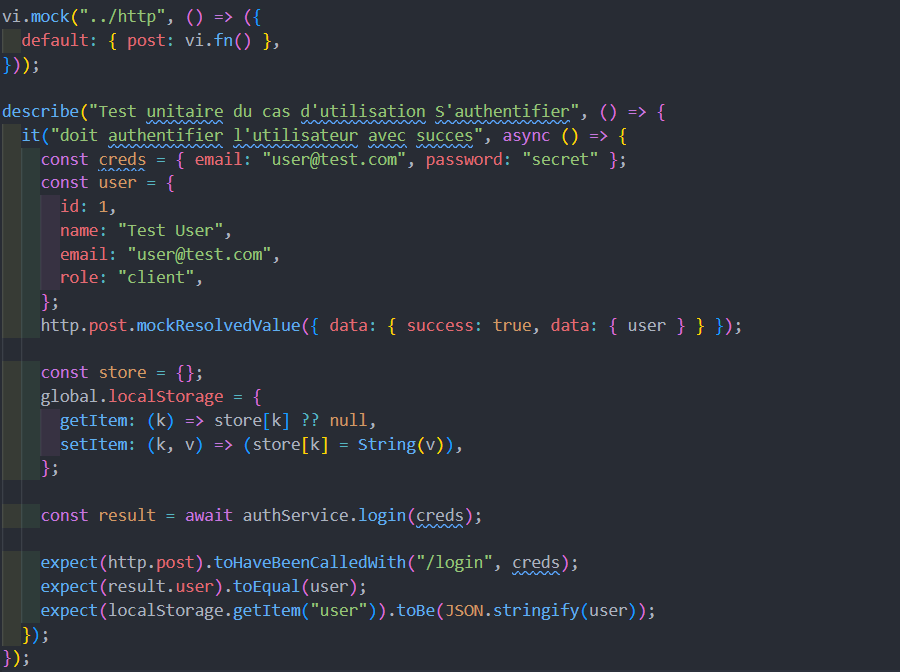
\includegraphics[width=0.9\linewidth]{Chapitres/Figures/test1_code.png}
    \caption{Test unitaire du cas d’utilisation «S’authentifier»}
\end{figure}


\subsection{Test unitaire du cas d’utilisation «Bloquer ou Débloquer une agence»}

Cette section se concentre sur la récupération du code pour le cas Bloquer ou
Débloquer une agence.

\subsection*{- Code source de la méthode de blocage ou déblocage d'une agence :}

\begin{figure}[H]
    \centering
    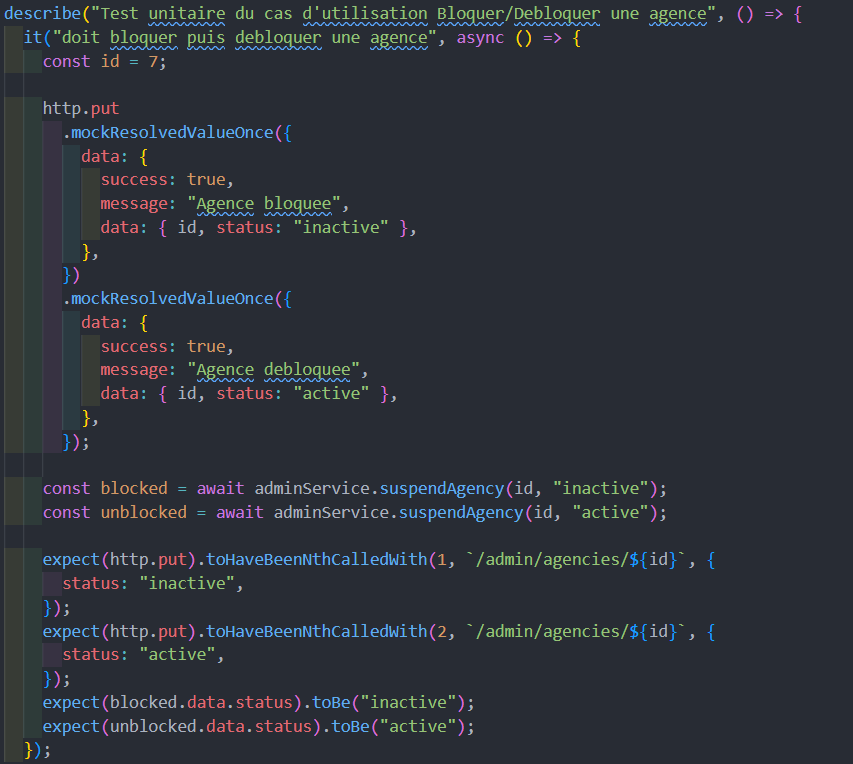
\includegraphics[width=0.9\linewidth]{Chapitres/Figures/test2_code.png}
    \caption{Test unitaire du cas d’utilisation «Bloquer ou Débloquer un agence»}
\end{figure}




%%%%%%%%%%%%%%%%%%%%%%%%%%%%%%%%%%%%%%%%%%%%%%%%%%%%%%%%%%%%%%%%%%%%%%%%%%%%%%%%%%%%%%%%%%%%%%%%%%%%%%%%%%%%
\section{Conclusion}
%%%%%%%%%%%%%%%%%%%%%%%%%%%%%%%%%%%%%%%%%%%%%%%%%%%%%%%%%%%%%%%%%%%%%%%%%%%

Dans le cadre de ce chapitre, nous avons mené le Sprint 1 selon une séquence logique couvrant l'analyse des cas d'utilisation, la conception et les tests. La phase suivante concerne la mise en œuvre du Sprint 2, qui est dédié à la gestion des réservations, des réclamations et du tableau de bord.